\documentclass[10pt,openright,twosides]{report}
\usepackage{geometry}                % See geometry.pdf to learn the layout options. There are lots.
\geometry{a4paper}                   % ... or a4paper or a5paper or ... 
%\geometry{landscape}                % Activate for for rotated page geometry
%\usepackage[parfill]{parskip}    % Activate to begin paragraphs with an empty line rather than an indent
\usepackage[utf8]{inputenc}
\usepackage{newunicodechar}
\usepackage{graphicx}
\usepackage{amssymb}
\usepackage{epstopdf}
\usepackage{listings}
\usepackage{longtable}
\usepackage{colortbl}
\usepackage[table]{xcolor}
\usepackage{underscore}
\usepackage{xcolor}
\usepackage{tikzpagenodes}
\usepackage{eso-pic}
\usepackage{hyperref}

\usetikzlibrary{calc}
\usetikzlibrary{positioning}
\usepgflibrary{shapes.geometric}
\usetikzlibrary{shapes.misc}
\usetikzlibrary{arrows}

%\usepackage{fontspec}
%\setmainfont{Verdana}[Ligatures=TeX]
%\setsansfont{Courier}[Ligatures=NoCommon]
%\setmonofont{Menlo}[Ligatures=NoCommon]

%
%\AddToShipoutPictureBG{%
%\begin{tikzpicture}[overlay,remember picture]
%\draw[line width=0.5pt]
%      ($ (current page text area.north west) $)
%      rectangle
%      ($ (current page text area.south east) $);
%\end{tikzpicture}
%}

\makeatletter
\newcommand*{\pmzeroslash}{%
  \nfss@text{%
    \sbox0{0}%
    \sbox2{/}%
    \sbox4{%
      \raise\dimexpr((\ht0-\dp0)-(\ht2-\dp2))/2\relax\copy2 %
    }%
    \ooalign{%
      \hfill\copy4 \hfill\cr
      \hfill0\hfill\cr
    }%
    \vphantom{0\copy4 }% correct overall height and depth of the symbol
  }%
}
\makeatother



\definecolor{seagreen}{RGB}{64,100,120}
\definecolor{darkpink}{RGB}{200,100,120}
\definecolor{light-gray}{gray}{0.85}
\definecolor{medium-gray}{gray}{0.5}
\definecolor{light-blue}{RGB}{240,240,255}
\definecolor{medium-marroon}{RGB}{200,100,0} 
\definecolor{light-yellow}{RGB}{255,255,200} 
\definecolor{light-green}{RGB}{200,255,200} 

\DeclareGraphicsRule{.tif}{png}{.png}{`convert #1 `dirname #1`/`basename #1 .tif`.png}

\lstdefinelanguage{gtl}
{
  morekeywords= {
	  import,
	  func,
	  getter,
	  setter,
	  after,
	  before,
	  between,
	  default,
	  do,
	  down,
	  up,
	  else,
	  elsif,
	  emptylist,
	  emptymap,
	  end,
	  error,
	  exists,
	  false,
	  for,
	  foreach,
	  from,
	  here,
	  unlet,
	  let,
	  loop,
	  no,
	  if,
	  in,
	  mod,
	  not,
	  or,
	  step,
	  template,
	  then,
	  to,
	  true,
	  yes,
	  warning,
	  while,
	  write,
	  display,
	  print,
	  println,
	  repeat,
	  input,
	  tab,
	  !,
	  ?,
	  isANumber,
	  description,
	  setDescription,
	  type,
	  touch,
	  string,
	  hexString,
	  xString,
	  numberOfBytes,
	  signedNumberOfBytes,
	  numberOfBits,
	  signedNumberOfBits,
	  sign,
	  fitsUnsignedInByte,
	  fitsSignedInByte,
	  fitsUnsignedInWord,
	  fitsSignedInWord,
	  fitsUnsignedInLong,
	  fitsSignedInLong,
	  fitsUnsignedInLongLong,
	  fitsSignedInLongLong,
	  abs,
	  bitAtIndex,
	  setBitAtIndex,
	  complementBitAtIndex,
	  majorVersion,
	  minorVersion,
	  revision,
	  max8bitsUnsignedInt,
	  max8bitsSignedInt,
	  min8bitsSignedInt,
	  max16bitsUnsignedInt,
	  max16bitsSignedInt,
	  min16bitsSignedInt,
	  max32bitsUnsignedInt,
	  max32bitsSignedInt,
	  min32bitsSignedInt,
	  max64bitsUnsignedInt,
	  max64bitsSignedInt,
	  min64bitsSignedInt,
	  isAlnum,
	  isAlpha,
	  isDigit,
	  isCntrl,
	  isLower,
	  isUpper,
	  isXDigit,
	  cos,
	  sin,
	  tan,
	  cosDegree,
	  sinDegree,
	  tanDegree,
	  exp,
	  logn,
	  log2,
	  log10,
	  sqrt,
	  power,
	  charAtIndex,
	  indexOfChar,
	  indexOfCharInRange,
	  containsChar,
	  containsCharInRange,
	  HTMLRepresentation,
	  identifierRepresentation,
	  fileExists,
	  length,
	  lowercaseString,
	  capitalized,
	  uppercaseString,
	  leftSubString,
	  rightSubString,
	  subString,
	  reversedString,
	  componentsSeparatedByString,
	  columnPrefixedBy,
	  wrap,
	  subStringExists,
	  replaceString,
	  envVar,
	  envVarExists,
	  setCharAtIndex,
	  version,
	  currentDir,
	  homeDir,
	  currentDateTime,
	  trueFalse,
	  TrueFalse,
	  yesNo,
	  TRUEFALSE,
	  trueOrFalse,
	  yesOrNo,
	  TRUEOrFALSE,
	  YESOrNO,
	  int,
	  map,
	  first,
	  last,
	  mapBy,
	  subListTo,
	  subListFrom,
	  subList,
	  insert,
	  list,
	  executable,
	  variables,
	  getter,
	  setter,
	  self,
	  typeof,
	  mapof,
	  listof,
	  by,
	  sort
	},
  emph={
    condition,
    var,
    variable,
    expression,
    expression_start,
    expression_end,
    increment,
    literal_string,
    instruction_list,
    instruction_list_1,
    instruction_list_2,
    template_file_name,
    aGetter,
    aSetter,
    hierarchy,
    index_var,
    key,
    limit_expression,
    extension,
    file_reference,
    argument_list,
    formal_argument_list,
    func_name,
    getter_name,
    setter_name,
    result_var,
    a_type,
    identifier
  },
  emphstyle=\em,
  moredelim=[s][\color{blue}]{\%}{\%},
  moredelim=[s][\color{seagreen}]{"}{"},
  morecomment=[l][\color{medium-marroon}\itshape]{\#},
  basicstyle=\ttfamily\footnotesize,
  morekeywords=\bfseries,
  backgroundcolor=\color{light-blue},
  rulecolor=\color{light-blue},
  xleftmargin=0.5em,
  xrightmargin=0.5em,
  frame=single,
  framesep=0.5em
}

\lstdefinelanguage{gtl-tmode}
{
  basicstyle=\ttfamily\footnotesize\color{blue},
  backgroundcolor=\color{light-blue},
  rulecolor=\color{light-blue},
  xleftmargin=0.5em,
  xrightmargin=0.5em,
  frame=single,
  framesep=0.5em
}

\lstdefinelanguage{console}{
  breaklines=true,
  basicstyle=\ttfamily\footnotesize,
  backgroundcolor=\color{light-yellow},
  rulecolor=\color{light-yellow},
  xleftmargin=0.5em,
  xrightmargin=0.5em,
  frame=single,
  framesep=0.5em
}  

\lstdefinelanguage{output}{
  basicstyle=\ttfamily\footnotesize,
  backgroundcolor=\color{light-green},
  rulecolor=\color{light-green},
  xleftmargin=0.5em,
  xrightmargin=0.5em,
  frame=single,
  framesep=0.5em
}  


\lstnewenvironment{gtl}{\lstset{language=gtl}}{}
\lstnewenvironment{gtl-tmode}{\lstset{language=gtl-tmode}}{}
\lstnewenvironment{console}{\lstset{language=console}}{}
\lstnewenvironment{templateoutput}{\lstset{language=output}}{}

\newcommand{\character}[1]{{\small\ttfamily `{#1}'}}

\newcommand{\argu}[1]{{\ttfamily #1}}
\newcommand{\ctype}[1]{{\small\ttfamily #1}}
\newcommand{\gtltype}[1]{{\small\ttfamily #1}}
\newcommand{\cdata}[1]{{\ttfamily #1}}
\newcommand{\var}[1]{{\small\ttfamily #1}}
\newcommand{\va}{\small\ttfamily\em}
\newcommand{\cfunction}[1]{{\ttfamily #1}}
\newcommand{\cmacro}[1]{{\small\ttfamily #1}}
\newcommand{\constant}[1]{{\small\ttfamily #1}}
\newcommand{\oilobj}[1]{{\small\ttfamily #1}}
\newcommand{\oilattr}[1]{{\small\ttfamily #1}}
\newcommand{\oilval}[1]{{\small\ttfamily #1}}
\newcommand{\member}[1]{{\small\ttfamily #1}}
\newcommand{\mem}{\small\ttfamily}
\newcommand{\tool}[1]{{\em #1}}
\newcommand{\na}{\scriptsize\ttfamily NA}

\newcommand{\icst}[1]{{\footnotesize\ttfamily\colorbox{light-blue}{#1}}}
\newcommand{\ccst}[1]{{\footnotesize\ttfamily\colorbox{light-blue}{'#1'}}}
\newcommand{\scst}[1]{{\footnotesize\ttfamily\colorbox{light-blue}{"#1"}}}
\newcommand{\gtlarg}[1]{{\footnotesize\ttfamily\colorbox{light-blue}{#1}}}

\newcommand{\gtlinline}[1]{\colorbox{light-blue}{\lstinline[language=gtl]{#1}}}

\newcommand{\example}{\vspace{.75em}\noindent\textbf{Example}\vspace{0em}}
\newcommand{\examplen}[1]{\vspace{.75em}\noindent\textbf{Example #1}\vspace{0em}}
\newcommand{\exampleof}[1]{\vspace{.5em}\noindent\textbf{Example of #1}\vspace{.5em}}
\newcommand{\outputs}{\vspace{.5em}\noindent\textbf{prints}\vspace{.5em}}

\renewcommand{\ttdefault}{pcr}

\newcommand\Warning{%
 \makebox[1.4em][c]{%
 \makebox[0pt][c]{\raisebox{-.05em}{\scriptsize!}}%
 \makebox[0pt][c]{\raisebox{-.2em}{\color{red}\Large$\bigtriangleup$}}}}%

\newcommand{\warning}[1]{%
\vspace{1em}
\hspace{-18.3mm}
\rowcolors{1}{white}{light-gray}
\begin{tabular}[b]{m{5mm}|m{\linewidth}}
\Warning & #1\\
\end{tabular}
}


\title{GTL Template language}
\author{Jean-Luc B\'echennec}
%\date{}                                           % Activate to display a given date or no date

\begin{document}

\maketitle
%\section{}
%\subsection{}

\tableofcontents

\chapter{About this document}

This document presents the syntax and the semantics of GTL 3, a template language used in Goil, the OIL compiler of Trampoline\footnote{An OSEK and AUTOSAR 4.2 compliant RTOS, check \url{https://github.com/TrampolineRTOS/trampoline}.}, to generate code from the OIL or arXML description of an OSEK/AUTOSAR application.

GTL is written in GalGas 3\,\footnote{GalGas 3 is free software distributed under the GPL license and can be found at \url{http://galgas.rts-software.org}}, a lexical and syntactic analyzer, which is also a powerful domain specific language to write compilers and interpreters. GalGas 3 is developed by Pierre Molinaro from the Real-Time Systems Group of IRCCyN, a french laboratory from a joint of the University of Nantes, \'Ecole Centrale de Nantes, \'Ecole des Mines de Nantes and CNRS. The first version of the GTL interpreter was written by Pierre Molinaro too. As needs increases, more features was needed and this led to a major rewrite of the GTL interpreter; In fact no original code made its way in GTL 3.

\section*{Convention}

Code examples follow the following conventions:
\begin{itemize}
\item GTL example code snippets are presented in \colorbox{light-blue}{light blue boxes}. In these examples, {\em Italic} writing are used for generic syntactic items. For instance, \gtlinline{expression} means any expression like \gtlinline{a + b} or \gtlinline{"a string"}. Boldface words are reserved words of GTL, like \gtlinline{foreach} or built-in functions, getters or setters like \gtlinline{setDescription}. Pieces of code delimited by \gtlinline{<} and \gtlinline{>} are optional.
\item Standard output of examples are presented in \colorbox{light-yellow}{light yellow boxes}.
\item Template string output of examples are presented in \colorbox{light-green}{light green boxes}.
\end{itemize}

%\newpage
\chapter{Data types}

GTL supports the following data types:
\rowcolors{1}{white}{light-gray}
\begin{longtable}{>{\bfseries\ttfamily\small}l|l}
{\bf type}&{\bf Description}\\
\hline\endhead
 {int}&
  {arbitrary precision integer numbers. The GMP library is used}\\
 {char}&
  {unicode chars}\\
 {float}&
  {64 bits floating point numbers}\\
 {bool}&
  {standard boolean}\\
 {enum}&
  {enumerated type}\\
 {string}&
  {unicode strings}\\
 {struct}&
  {structured data}\\
 {list}&
  {lists of data, may be accessed as a table}\\
 {map}&
  {map (aka dictionary) of data}\\
 {type}&
  {the type of a data}\\
 {unconstructed}&
  {an unconstructed variable}
\end{longtable}

Data embed a location, that is a file name, a line and a column. Each time a variable is set, the corresponding location is set too. This allow to report errors efficiently. See \ref{sec:touch} and \ref{sec:warningInstruction}.

Data embed a description string too. This allow to comment on the content of the data. See \ref{sec:description} and \ref{sec:setDescription}.

Each type has its set of operators, getters and setters. The expression, for getters, or the variable, for setters, is called the {\em target}. Getters return a value related to the expression but do not change it. They are used to get information from a data or to convert it into another type.  Setters may only target a variable. Setters change the content of the variable and do not return anything. Getters and setters may have arguments. Syntax for getters without argument is as follow:

\begin{gtl}
[expression aGetter]
\end{gtl}

When the getter takes arguments, they are listed after a colon and separated commas as follow:

\begin{gtl}
[expression aGetter : arg1, arg2, ..., argN]
\end{gtl}

Syntax for setters without arguments is as follow:

\begin{gtl}
[!variable aSetter]
\end{gtl}

When the setter takes arguments, they are listed after a colon and separated by commas as follow:

\begin{gtl}
[!variable aSetter : arg1, arg2, ..., argN]
\end{gtl}

%==============================================================================================
\section{Operators priority}

The following table gives all the operators available in GTL an their priority. Semantics of the operators is given for each data type. Operators of same priority are evaluated from left to right.

\rowcolors{1}{white}{light-gray}
\begin{longtable}{l|>{\ttfamily}l}
{\bf Priority}&{\bf Operators}\\
\hline\endhead
 {0}&
  {| \^{}}\\
 {1}&
  {\&}\\
 {2}&
  {== != < > <= >=}\\
 {3}&
  {<< >> + . -}\\
 {4}&
  {* / mod}\\
 {5}&
  {not \raisebox{-1mm}{\textasciitilde} - +}\\
\end{longtable}

\section{Special operators}

\subsection{The \texttt{exists} operator}

The \gtlinline{exists} operator tests the existence of a variable, a struct field,  an item of a map or a list and returns a bool, \gtlinline{true} if the entity exists, \gtlinline{false} otherwise.

\begin{gtl}
exists var
\end{gtl}

\example
\begin{gtl}
let c := 3
if exists c then println "c exists" else println "c does not exist" end if
unlet c # delete c
if exists c then println "c exists" else println "c does not exist" end if
\end{gtl}
\begin{console}
c exists
c does not exist
\end{console}

\subsection{The \texttt{exists \ldots{} default (\ldots)} operator}

The \gtlinline{exists ... default (...)} operator tests the existence of a variable, a struct field,  an item of a map or a list.

\begin{gtl}
exists var default ( expression )
\end{gtl}

If the entity exists it is returned. Otherwise the evaluation of the default expression is returned.

\example
\begin{gtl}
let aList := @( 1, 2, 3 )
let aSecondList := exists aList default ( @() )
display aSecondList
unlet aList # delete aList
let aSecondList := exists aList default ( @() )
display aSecondList
\end{gtl}
\begin{console}
aSecondList from file '/Users/jlb/Develop/GTL/examples/testTypes.gtl', line 9:7
  - list: @(
    0 :>
        integer: 1
    1 :>
        integer: 2
    2 :>
        integer: 3
)
aSecondList from file '/Users/jlb/Develop/GTL/examples/testTypes.gtl', line 12:7
  - list: @(
)
\end{console}

\subsection{The \texttt{typeof} operator}

The \gtlinline{typeof} operator takes a variable as argument an return its type.

\begin{gtl}
typeof var
\end{gtl}

\warning{The \gtlinline{typeof} is deprecated. Use the \gtlinline{type} getter instead. See \ref{sec:type}.}

\subsection{The \texttt{mapof} operator}

The \gtlinline{mapof} may apply on \gtltype{struct} or on \gtltype{list}.

\subsubsection{With a \texttt{struct}}

The \gtlinline{mapof} operator converts a \gtltype{struct} to a \gtltype{map}.

\begin{gtl}
mapof expression end
\end{gtl}

\warning{\gtlinline{mapof} is deprecated, use the map getter on \gtltype{struct} instead. See \ref{sec:mapGetterOnStruct}.}

\example 
\begin{gtl}
let aStruct := @{ a: 1, b: 2, c: 3 }
display aStruct
let aMap := mapof aStruct end
display aMap
\end{gtl}
\begin{console}
aStruct from file '/Users/jlb/Develop/GTL/examples/mapofTest.gtl', line 3:7
  - struct: @{
    a :>
        integer: 1
    b :>
        integer: 2
    c :>
        integer: 3
}
aMap from file '/Users/jlb/Develop/GTL/examples/mapofTest.gtl', line 5:7
  - map: @[
    "a" :>
        integer: 1
    "b" :>
        integer: 2
    "c" :>
        integer: 3
]
\end{console}

\subsubsection{With a \texttt{list}}

The \gtlinline{mapof} operator converts a \gtltype{list} to a \gtltype{map} according to a \gtltype{string} field of each item of the \gtltype{list}. So the list should be a \gtltype{list} of \gtltype{struct}.

\begin{gtl}
mapof var by identifier
\end{gtl}

\warning{\gtlinline{mapof ... by} is deprecated, use the \gtlinline{mapBy} getter on \gtltype{list} instead. See \ref{sec:mapByGetterOnList}.}

\example
\begin{gtl}
let aList := @(
  @{ age : 18, height : 180, name : "Arnold" },
  @{ age : 22, height : 170, name : "Bob"    },
  @{ age : 29, height : 175, name : "John"   }
)
let aMap := mapof aList by name
display aMap
\end{gtl}
\begin{console}
aMap from file '/Users/jlb/Develop/GTL/examples/mapofTest.gtl', line 13:7
  - map: @[
    "Arnold" :>
        struct: @{
            age :>
                integer: 18
            height :>
                integer: 180
            name :>
                string: "Arnold"
        }
    "Bob" :>
        struct: @{
            age :>
                integer: 22
            height :>
                integer: 170
            name :>
                string: "Bob"
        }
    "John" :>
        struct: @{
            age :>
                integer: 29
            height :>
                integer: 175
            name :>
                string: "John"
        }
]
\end{console}

\subsection{The \texttt{listof} operator}

The \gtlinline{listof} operator apply to a \gtltype{map} variable. It returns a \gtltype{list} representation of the \gtltype{map}. The elements of the \gtltype{list} are sorted in the alphanumerical order of the \gtltype{map} keys.

\begin{gtl}
listof var end
\end{gtl}

\warning{\gtlinline{listof ... by} is deprecated, use the \gtlinline{list} getter on \gtltype{map} instead. See \ref{sec:listGetterOnMap}.}


%==============================================================================================
\section{Getters applicable to any data type}

\subsection{The \texttt{type} getter} 
\label{sec:type}

The \gtlinline{type} getter returns the type of the expression. See the section \ref{sec:typetype}.

\example

\begin{gtl}
let a := 1
let typeOfA := [a type]
display typeOfA
\end{gtl}

\begin{console}
typeOfA from file '/Users/jlb/Develop/GTL/examples/testTypes.gtl', line 4:7
  - type: int
\end{console}

\subsection{The \texttt{isANumber} getter} 
\label{sec:isANumber}
 
\gtlinline{isANumber} returns \gtlinline{true} if the expression is a number: \gtltype{int} or \gtltype{float}, \gtlinline{false} otherwise. This getter is useful to test the type of an argument in a function, a getter or a setter.

\example

\begin{gtl}
let b := 0
let a := 1
if [a isANumber] then
  let b := a # if a is a number, it is copied in b
else
  let b := 0 # otherwise b is set to 0
end if
display b
\end{gtl}

\begin{console}
b from file '/Users/jlb/Develop/GTL/examples/testTypes.gtl', line 13:7
  - integer: 1
\end{console}


\subsection{The \texttt{description} getter} 
\label{sec:description}

\gtlinline{description} returns the string describing the data, if available, or an empty string otherwise. If the data is coming from an OIL source file, it corresponds to the description field (see section 2.3.11 of \emph{System Generation -- OIL: OSEK Implementation Language -- Version 2.5}).

\section{Setters applicable to any data type}

\subsection{The \texttt{setDescription} setter} 
\label{sec:setDescription}

\gtlinline{setDescription} takes one string argument \lstinline[language=gtl]{desc}. It sets the string describing the data to \lstinline[language=gtl]{desc}.

\subsection{The \texttt{touch} setter} 
\label{sec:touch}

\gtlinline{touch} sets the location of modification of the data to the current one.

\section{The \texttt{int} data type}

The \gtltype{int} data type support arbitrary precision arithmetic by using the GNU Multiple Precision Arithmetic Library (GMP).

\subsection{The \texttt{int} operators}

The \lstinline{int} datatype supports the following operators:

\subsubsection{Unary operators}

\rowcolors{1}{white}{light-gray}
\begin{longtable}{>{\ttfamily}l|>{\ttfamily}l|l}
{\bf Operator}&{\bf Expression type}&{\bf Meaning}\\
\hline\endhead
 {+}&
  {int $\leftarrow$ +int}&
  {Plus operator. No effect}\\
 {-}&
  {int $\leftarrow$ -int}&
  {Minus operator. Negation}\\
 {\raisebox{-1.2mm}{\textasciitilde}}&
  {int $\leftarrow$ \raisebox{-1.2mm}{\textasciitilde}int}&
  {Not operator. Complementation by 1}\\
\end{longtable}

\subsubsection{Binary arithmetic operators}

\rowcolors{1}{white}{light-gray}
\begin{longtable}{>{\ttfamily}l|>{\ttfamily}l|l}
{\bf Operator}&{\bf Expression type}&{\bf Meaning}\\
\hline\endhead
 {+}&
  {int $\leftarrow$ int + int}&
  {Addition}\\
 {-}&
  {int $\leftarrow$ int - int}&
  {Substraction}\\
 {*}&
  {int $\leftarrow$ int * int}&
  {Multiplication}\\
 {/}&
  {int $\leftarrow$ int / int}&
  {Division}\\
 {mod}&
  {int $\leftarrow$ int mod int}&
  {Modulus}\\
\end{longtable}

\subsubsection{Binary bitwise operators}
\rowcolors{1}{white}{light-gray}
\begin{longtable}{>{\ttfamily}l|>{\ttfamily}l|l}
{\bf Operator}&{\bf Expression type}&{\bf Meaning}\\
\hline\endhead
 {\&}&
  {int $\leftarrow$ int \& int}&
  {bitwise and}\\
 {|}&
  {int $\leftarrow$ int | int}&
  {bitwise or}\\
 {\^~}&
  {int $\leftarrow$ int \^{} int}&
  {bitwise exclusive or}\\
 {<<}&
  {int $\leftarrow$ int << int}&
  {shift left}\\
 {>>}&
  {int $\leftarrow$ int >> int}&
  {shift right}\\
\end{longtable}

\subsubsection{Comparison operators}

\rowcolors{1}{white}{light-gray}
\begin{longtable}{>{\ttfamily}l|>{\ttfamily}l|l}
{\bf Operator}&{\bf Expression type}&{\bf Meaning}\\
\hline\endhead
 {!=}&
  {bool $\leftarrow$ int != int}&
  {Not equal}\\
 {==}&
  {bool $\leftarrow$ int == int}&
  {Equal}\\
 {>}&
  {bool $\leftarrow$ int > int}&
  {Greater than}\\
 {<}&
  {bool $\leftarrow$ int < int}&
  {Lower than}\\
 {>=}&
  {bool $\leftarrow$ int >= int}&
  {Greater or equal}\\
 {<=}&
  {bool $\leftarrow$ int <= int}&
  {Lower or equal}\\
\end{longtable}

\subsection{The \texttt{int} getters}

\subsubsection{The {\bfseries\ttfamily string} getter}

\gtlinline{string} returns a string decimal representation of the \gtltype{int} expression. 

\example
\begin{gtl}
let b := [42 string]
display b
\end{gtl}
\begin{console}
b from file '/Users/jlb/Develop/GTL/examples/testTypes.gtl', line 18:7
  - string: "42"
\end{console}


\subsubsection{The {\bfseries\ttfamily hexString} getter}

\gtlinline{hexString} returns a hexadecimal string representation of the int expression prefixed by \scst{0x}. If the int expression is negative a \ccst{-} is inserted before.

\example
\begin{gtl}
let a := [42 hexString]
display a
let b := [-20 hexString]
display b
\end{gtl}
\begin{console}
a from file '/Users/jlb/Develop/GTL/examples/testTypes.gtl', line 21:7
  - string: "0x2A"
b from file '/Users/jlb/Develop/GTL/examples/testTypes.gtl', line 23:7
  - string: "-0x14"
\end{console}

\subsubsection{the {\bfseries\ttfamily xString} getter}

\gtlinline{xString} returns a hexadecimal string representation of the int expression. If the expression is negative a \ccst{-} is inserted before.

\example
\begin{gtl}
let a := [42 xString]
display a
let b := [-20 xString]
display b
\end{gtl}
\begin{console}
a from file '/Users/jlb/Develop/GTL/examples/testTypes.gtl', line 26:7
  - string: "2A"
b from file '/Users/jlb/Develop/GTL/examples/testTypes.gtl', line 28:7
  - string: "-14"
\end{console}

\subsubsection{The {\bfseries\ttfamily numberOfBytes} getter}

\gtlinline{numberOfBytes} returns an int, the number of bytes needed to store an unsigned expression.

\example
\begin{gtl}
println [255 numberOfBytes]
println [256 numberOfBytes]
\end{gtl}
\begin{console}
1
2
\end{console}

\subsubsection{The {\bfseries\ttfamily signedNumberOfBytes} getter}

\gtlinline{signedNumberOfBytes} returns an int, the number of bytes needed to store a signed expression. 

\example
\begin{gtl}
println [127 signedNumberOfBytes]
println [128 signedNumberOfBytes]
\end{gtl}
\begin{console}
1
2
\end{console}

\subsubsection{The \texttt{numberOfBits} getter}

\gtlinline{numberOfBits} returns an int, the number of bits needed to store an unsigned expression.

\example
\begin{gtl}
println [63 numberOfBits]
println [64 numberOfBits]
\end{gtl}
\begin{console}
6
7
\end{console}


\subsubsection{The \texttt{signedNumberOfBits} getter}

\gtlinline{signedNumberOfBits} returns an int, the number of bits needed to store a signed expression. 

\example
\begin{gtl}
println [63 signedNumberOfBits]
println [64 signedNumberOfBits]
\end{gtl}
\begin{console}
7
8
\end{console}

\subsubsection{The \texttt{sign} getter}

\gtlinline{sign} returns an int, \icst{-1} if the expression is strictly negative, \icst{0} if it is null and \icst{+1} if the expression is strictly positive.


\subsubsection{The \texttt{fitsUnsignedInByte} getter}

\gtlinline{fitsUnsignedInByte} returns a bool, \gtlinline{true} if the expression fits in an unsigned byte, \gtlinline{false} otherwise.

\subsubsection{The \texttt{fitsSignedInByte} getter}

\gtlinline{fitsSignedInByte} returns a bool, \gtlinline{true} if the expression fits in a signed byte, \gtlinline{false} otherwise.

\subsubsection{The \texttt{fitsUnsignedInWord} getter}

\gtlinline{fitsUnsignedInWord} returns a bool, \gtlinline{true} if the expression fits in an unsigned 16 bits word, \gtlinline{false} otherwise.

\subsubsection{The \texttt{fitsSignedInWord} getter}

\gtlinline{fitsSignedInWord} returns a bool, \gtlinline{true} if the expression fits in a signed 16 bits word, \gtlinline{false} otherwise.

\subsubsection{The \texttt{fitsUnsignedInLong} getter}

\gtlinline{fitsUnsignedInLong} returns a bool, \gtlinline{true} if the expression fits in an unsigned 32 bits long, \gtlinline{false} otherwise.

\subsubsection{The \texttt{fitsSignedInLong} getter}

\gtlinline{fitsSignedInLong} returns a bool, \gtlinline{true} if the expression fits in a signed 32 bits long, \gtlinline{false} otherwise.

\subsubsection{The \texttt{fitsUnsignedInLongLong} getter}

\gtlinline{fitsUnsignedInLongLong} returns a bool, \gtlinline{true} if the expression fits in an unsigned 64 bits long long, \gtlinline{false} otherwise.

\subsubsection{The \texttt{fitsSignedInLongLong} getter}

\gtlinline{fitsSignedInLongLong} returns a bool, \gtlinline{true} if the expression fits in a signed 64 bits long long, \gtlinline{false} otherwise.

\subsubsection{The \texttt{abs} getter}

\gtlinline{abs} returns an int, the absolute value of the expression.

\subsubsection{The \texttt{bitAtIndex} getter}

\gtlinline{bitAtIndex} takes one int argument: \gtlarg{index}. It returns \gtlinline{true} if the bit at index \gtlarg{index} is set and \gtlinline{false} otherwise. \gtlarg{index} 0 corresponds to the lowest significant bit. 

\example
\begin{gtl}
let a := [1 bitAtIndex: 0]
display a
\end{gtl}
\begin{console}
a from file '/Users/jlb/Develop/GTL/examples/testTypes.gtl', line 63:7
  - boolean: true
\end{console}

\subsection{The \texttt{int} setters}

\subsubsection{The \texttt{setBitAtIndex} setter}

\gtlinline{setBitAtIndex} takes two arguments. The first one, \gtlarg{value}, is a bool. The second one, \gtlarg{index}, is the index of the bit to set. if \gtlarg{value} is \gtlinline{true} the bit is set to \gtlinline{1} and to \gtlinline{0} otherwise.

\example
\begin{gtl}
let a := 0
[!a setBitAtIndex: true, 0]
display a
\end{gtl}
\begin{console}
a from file '/Users/jlb/Develop/GTL/examples/testTypes.gtl', line 64:7
  - integer: 1
\end{console}

\subsubsection{The \texttt{complementBitAtIndex} setter}

\gtlinline{complementBitAtIndex} takes one int argument, \gtlarg{index}, which is the index of the bit to complement. 

\example
\begin{gtl}
let a := 1
[!a complementBitAtIndex: true, 1]
display a
\end{gtl}
\begin{console}
a from file '/Users/jlb/Develop/GTL/examples/testTypes.gtl', line 68:7
  - integer: 3
\end{console}

\subsection{The \texttt{int} functions}

The following built-in functions return an int.

\subsubsection{The function \texttt{majorVersion()}}

\gtlinline{majorVersion()} takes no argument and returns the major version of the compiler in where GTL is embedded. For instance, if the version string is \scst{3.2.1}, it returns \icst{3}.

\subsubsection{The function \texttt{minorVersion()}}

\gtlinline{minorVersion()} takes no argument and returns the minor version of the compiler in where GTL is embedded. For instance, if the version string is \scst{3.2.1}, it returns \icst{2}.

\subsubsection{The function \texttt{revision()}}

\gtlinline{revision()} takes no argument and returns the revision of the compiler in where GTL is embedded. For instance, if the version string is \scst{3.2.1}, it returns \icst{1}.

\subsubsection{The function \texttt{max8bitsUnsignedInt()}}

\gtlinline{max8bitsUnsignedInt()} takes no argument and returns the maximum unsigned number that fits in 8 bits.

\subsubsection{The function \texttt{max8bitsSignedInt()}}

\gtlinline{max8bitsSignedInt()} takes no argument and returns the maximum signed number that fits in 8 bits.

\subsubsection{The function \texttt{min8bitsSignedInt()}}

\gtlinline{min8bitsSignedInt()} takes no argument and returns the minimum signed number that fits in 8 bits.

\subsubsection{The function \texttt{max16bitsUnsignedInt()}}

\gtlinline{max16bitsUnsignedInt()} takes no argument and returns the maximum unsigned number that fits in 16 bits.

\subsubsection{The function \texttt{max16bitsSignedInt()}}

\gtlinline{max16bitsSignedInt()} takes no argument and returns the maximum signed number that fits in 16 bits.

\subsubsection{The function \texttt{min16bitsSignedInt()}}

\gtlinline{min16bitsSignedInt()} takes no argument and returns the minimum signed number that fits in 16 bits.

\subsubsection{The function \texttt{max32bitsUnsignedInt()}}

\gtlinline{max32bitsUnsignedInt()} takes no argument and returns the maximum unsigned number that fits in 32 bits.

\subsubsection{The function \texttt{max32bitsSignedInt()}}

\gtlinline{max32bitsSignedInt()} takes no argument and returns the maximum signed number that fits in 32 bits.

\subsubsection{The function \texttt{min32bitsSignedInt()}}

\gtlinline{min32bitsSignedInt()} takes no argument and returns the minimum signed number that fits in 32 bits.

\subsubsection{The function \texttt{max64bitsUnsignedInt()}}

\gtlinline{max64bitsUnsignedInt()} takes no argument and returns the maximum unsigned number that fits in 64 bits.

\subsubsection{The function \texttt{max64bitsSignedInt()}}

\gtlinline{max64bitsSignedInt()} takes no argument and returns the maximum signed number that fits in 64 bits.

\subsubsection{The function \texttt{min64bitsSignedInt()}}

\gtlinline{min64bitsSignedInt()} takes no argument and returns the minimum signed number that fits in 64 bits.

\section{The \texttt{char} data type}

The \lstinline{char} data type supports unicode characters. A literal char is delimited by a pair of \texttt{'}:

\begin{gtl}
let a := 'A'
\end{gtl}

Literal chars support escaped special characters:

\rowcolors{1}{white}{light-gray}
\begin{longtable}{>{\ttfamily}l|l}
{\bf Escape sequence}&{\bf Corresponding character}\\
\hline\endhead
 {\textbackslash f}&
  {form feed}\\
 {\textbackslash n}&
  {new line}\\
 {\textbackslash r}&
  {return}\\
 {\textbackslash t}&
  {horizontal tab}\\
 {\textbackslash v}&
  {vertical tab}\\
 {\textbackslash\textbackslash}&
  {backslash}\\
 {\textbackslash '}&
  {'}\\
 {\textbackslash\pmzeroslash}&
  {null character}\\
 {\textbackslash u\textsl{nnnn}}&
  {unicode character with code \textsl{nnnn} in hexadecimal}\\
 {\textbackslash U\textsl{nnnnnnnn}}&
  {unicode character with code \textsl{nnnnnnnn} in hexadecimal}\\
\end{longtable}

\subsection{The \texttt{char} operators}

The \lstinline{char} data type supports the following operators:

\subsubsection{Comparison operators}

\rowcolors{1}{white}{light-gray}
\begin{longtable}{>{\ttfamily}l|>{\ttfamily}l|l}
{\bf Operator}&{\bf Expression type}&{\bf Meaning}\\
\hline\endhead
 {!=}&
  {bool $\leftarrow$ char != char}&
  {Not equal}\\
 {==}&
  {bool $\leftarrow$ char == char}&
  {Equal}\\
 {>}&
  {bool $\leftarrow$ char > char}&
  {Greater than}\\
 {<}&
  {bool $\leftarrow$ char < char}&
  {Lower than}\\
 {>=}&
  {bool $\leftarrow$ char >= char}&
  {Greater or equal}\\
 {<=}&
  {bool $\leftarrow$ char <= char}&
  {Lower or equal}\\
\end{longtable}

\subsection{The \texttt{char} getters}

\subsubsection{The \texttt{string} getter}

\gtlinline{string} returns a string representation of the char expression. \gtlinline{['c' string]} returns string \scst{c}.

\subsubsection{The \texttt{isAlnum} getter}

\gtlinline{isAlnum} returns a bool, \gtlinline{true} if the char expression is an ASCII alphanumeric character: between \ccst{A} and \ccst{Z} or between \ccst{a} and \ccst{z} or between \ccst{0} and \ccst{9}, \gtlinline{false} otherwise.

\subsubsection{The \texttt{isAlpha} getter}

\gtlinline{isAlpha} returns a bool, \gtlinline{true} if the char expression is an ASCII letter: between \ccst{A} and \ccst{Z} or between \ccst{a} and \ccst{z}, \gtlinline{false} otherwise.

\subsubsection{The \texttt{isDigit} getter}

\gtlinline{isDigit} returns abool, \gtlinline{true} if the char expression is an ASCII digit: between \ccst{0} and \ccst{9}, \gtlinline{false} otherwise.

\subsubsection{The \texttt{isCntrl} getter}

\gtlinline{isCntrl} returns a bool, \gtlinline{true} if the char expression is an ASCII control character, i.e. strictly before the {\em SPACE} character, \gtlinline{false} otherwise.

\subsubsection{The \texttt{isLower} getter}

\gtlinline{isLower} returns a bool, \gtlinline{true} if the char expression is an ASCII lower case letter: between \ccst{a} and \ccst{z}, \gtlinline{false} otherwise.

\subsubsection{The \texttt{isUpper} getter}

\gtlinline{isUpper} returns a bool, \gtlinline{true} if the char expression is an ASCII upper case letter: between \ccst{A} and \ccst{Z} , \gtlinline{false} otherwise.

\subsubsection{The \texttt{isXDigit} getter}

\gtlinline{isXDigit} returns a bool, \texttt{true} if the char expression is an ASCII hexadecimal digit: between \ccst{A} and \ccst{F} or between \ccst{a} and \ccst{f} or between \ccst{0} and \ccst{9}, \texttt{false} otherwise.
  
\section{The \texttt{float} data type}

The \gtltype{float} data type is the standard IEEE784 64 bits floating point number.

\subsection{The \texttt{float} operators}

The \gtltype{float} data type supports the following operators:

\subsubsection{Unary operators}

\rowcolors{1}{white}{light-gray}
\begin{longtable}{>{\ttfamily}l|>{\ttfamily}l|l}
{\bf Operator}&{\bf Expression type}&{\bf Meaning}\\
\hline\endhead
 {+}&
  {float $\leftarrow$ +float}&
  {Plus operator. No effect}\\
 {-}&
  {float $\leftarrow$ -float}&
  {Minus operator. Negation}\\
\end{longtable}

\subsubsection{Binary arithmetic operators}

\rowcolors{1}{white}{light-gray}
\begin{longtable}{>{\ttfamily}l|>{\ttfamily}l|l}
{\bf Operator}&{\bf Expression type}&{\bf Meaning}\\
\hline\endhead
 {+}&
  {float $\leftarrow$ float + float}&
  {Addition}\\
 {-}&
  {float $\leftarrow$ float - float}&
  {Substraction}\\
 {*}&
  {float $\leftarrow$ float * float}&
  {Multiplication}\\
 {/}&
  {float $\leftarrow$ float / float}&
  {Division}\\
\end{longtable}

\subsubsection{Comparison operators}

\rowcolors{1}{white}{light-gray}
\begin{longtable}{>{\ttfamily}l|>{\ttfamily}l|l}
{\bf Operator}&{\bf Expression type}&{\bf Meaning}\\
\hline\endhead
 {!=}&
  {bool $\leftarrow$ float != float}&
  {Not equal}\\
 {==}&
  {bool $\leftarrow$ float == float}&
  {Equal}\\
 {>}&
  {bool $\leftarrow$ float > float}&
  {Greater than}\\
 {<}&
  {bool $\leftarrow$ float < float}&
  {Lower than}\\
 {>=}&
  {bool $\leftarrow$ float >= float}&
  {Greater or equal}\\
 {<=}&
  {bool $\leftarrow$ float <= float}&
  {Lower or equal}\\
\end{longtable}


\subsection{The \texttt{float} getters}

\subsubsection{The \texttt{string} getter}

\gtlinline{string} returns a string representation of the float expression. \gtlinline{[4.2 string]} returns string \scst{4.2}.
  
\subsubsection{The \texttt{cos} getter}

\gtlinline{cos} returns the cosine of a float expression expressed in radian.

\subsubsection{The \texttt{sin} getter}

\gtlinline{sin} returns the sine of a float expression expressed in radian.

\subsubsection{The \texttt{tan} getter}

\gtlinline{tan} returns the tangent of a float expression expressed in radian.

\subsubsection{The \texttt{cosDegree} getter}

\gtlinline{cosDegree} returns the cosine of a float expression expressed in degree.

\subsubsection{The \texttt{sinDegree} getter}

\gtlinline{sinDegree} returns the sine of a float expression expressed in degree.

\subsubsection{The \texttt{tanDegree} getter}

\gtlinline{tanDegree} returns the tangent of a float expression expressed in degree.

\subsubsection{The \texttt{exp} getter}

\gtlinline{exp} returns the exponentiation of a float expression.

\subsubsection{The \texttt{logn} getter}

\gtlinline{logn} returns the natural logarithm of a float expression.

\subsubsection{The \texttt{log2} getter}

\gtlinline{log2} returns the logarithm base 2 of a float expression.
  
\subsubsection{The \texttt{log10} getter}

\gtlinline{log10} returns the logarithm base 10 of a float expression.

\subsubsection{The \texttt{sqrt} getter}

\gtlinline{sqrt} returns the square root of a float expression.

\subsubsection{The \texttt{power} getter}

\gtlinline{power} takes one \gtltype{float} argument, \gtlarg{p}. It returns the expression raised to the  power of \gtlarg{p}.

\subsection{The \texttt{float} function}

The following function returns a \gtltype{float}

\subsubsection{The \texttt{pi()} function}

\gtlinline{pi()} returns an approximation of the $\pi$ constant value (3.141\allowbreak592\allowbreak653\allowbreak589\allowbreak793\allowbreak238\allowbreak462\allowbreak643\allowbreak383\allowbreak279\allowbreak502\allowbreak88).

\section{The \texttt{string} data type}

The \gtltype{string} data type supports unicode. A literal string is delimited by a pair of \texttt{"}.

\begin{gtl}
let a := "A literal string"
\end{gtl}

Literal strings support escaped special characters:

\rowcolors{1}{white}{light-gray}
\begin{longtable}{>{\ttfamily}l|l}
{\bf Escape sequence}&{\bf Corresponding character}\\
\hline\endhead
 {\textbackslash f}&
  {form feed}\\
 {\textbackslash n}&
  {new line}\\
 {\textbackslash r}&
  {return}\\
 {\textbackslash t}&
  {horizontal tab}\\
 {\textbackslash v}&
  {vertical tab}\\
 {\textbackslash\textbackslash}&
  {backslash}\\
 {\textbackslash '}&
  {'}\\
 {\textbackslash "}&
  {"}\\
 {\textbackslash\pmzeroslash}&
  {null character}\\
 {\textbackslash u\textsl{nnnn}}&
  {unicode character with code \textsl{nnnn} in hexadecimal}\\
 {\textbackslash U\textsl{nnnnnnnn}}&
  {unicode character with code \textsl{nnnnnnnn} in hexadecimal}\\
\end{longtable}

\subsection{The \texttt{string} operators}


The \gtltype{string} data type supports the following operators:

\subsubsection{Binary operator}

\rowcolors{1}{white}{light-gray}
\begin{longtable}{>{\ttfamily}l|>{\ttfamily}l|l}
{\bf Operator}&{\bf Expression type}&{\bf Meaning}\\
\hline\endhead
 {+}&
  {string $\leftarrow$ string + string}&
  {Concatenation}\\
\end{longtable}

\subsubsection{Comparison operators}

\rowcolors{1}{white}{light-gray}
\begin{longtable}{>{\ttfamily}l|>{\ttfamily}l|l}
{\bf Operator}&{\bf Expression type}&{\bf Meaning}\\
\hline\endhead
 {!=}&
  {bool $\leftarrow$ string != string}&
  {Not equal}\\
 {==}&
  {bool $\leftarrow$ string == string}&
  {Equal}\\
 {>}&
  {bool $\leftarrow$ string > string}&
  {Greater than}\\
 {<}&
  {bool $\leftarrow$ string < string}&
  {Lower than}\\
 {>=}&
  {bool $\leftarrow$ string >= string}&
  {Greater or equal}\\
 {<=}&
  {bool $\leftarrow$ string <= string}&
  {Lower or equal}\\
\end{longtable}


\subsection{The \texttt{string} getters}

\subsubsection{The \texttt{charAtIndex} getter}

\gtlinline{charAtIndex} takes one int argument, the \gtlarg{index}. It returns a char, the character at index \gtlarg{index}. The first char is at index 0, the last char is at index length of the string minus 1. If \gtlarg{index} is greater or equal than the length of the target, a run time error occurs.

\example
\begin{gtl}
let a := ["Hello" charAtIndex: 1]
display a
\end{gtl}
\begin{console}
a from file '/Users/jlb/Develop/GTL/examples/testTypes.gtl', line 74:7
  - char: e
\end{console}


\subsubsection{The \texttt{indexOfChar} getter}

\gtlinline{indexOfChar} takes one char argument, the \gtlarg{character} to look up. It returns an int, the index of the first occurrence of \gtlarg{character} in the target. If \gtlarg{character} is not found in the target, \icst{-1} is returned.

\example
\begin{gtl}
let a := ["Hello" indexOfChar: 'l']
let b := ["Hello" indexOfChar: 'z']
display a
display b
\end{gtl}
\begin{console}
a from file '/Users/jlb/Develop/GTL/examples/testTypes.gtl', line 78:7
  - integer: 2
b from file '/Users/jlb/Develop/GTL/examples/testTypes.gtl', line 79:7
  - integer: -1
\end{console}

\subsubsection{The \texttt{indexOfCharInRange} getter}

\gtlinline{indexOfCharInRange} takes two char argument, \gtlarg{minChar} and \gtlarg{maxChar} which define the character range to look up. It returns an int, the index of the first occurrence of the character being in range (bounds included) in the target. If \gtlarg{character} is not found in the target, \icst{-1} is returned.

\example
\begin{gtl}
let a := ["Hello" indexOfCharInRange: 'a', 'e']
display a
\end{gtl}
\begin{console}
a from file '/Users/jlb/Develop/GTL/examples/testTypes.gtl', line 82:7
  - integer: 1
\end{console}

\subsubsection{The \texttt{containsChar} getter}

\gtlinline{containsChar} takes one char argument, the \gtlarg{character} to look up. It returns a bool, \gtlinline{true} is the target contains the \gtlarg{character}, \gtlarg{false} otherwise.

\subsubsection{The \texttt{containsCharInRange} getter}

\gtlinline{containsCharInRange} takes two char argument, \gtlarg{minChar} and \gtlarg{maxChar} which define the character range to look up. It returns a bool, \texttt{true} is the target contains a character within the range (bounds included), \texttt{false} otherwise.

\subsubsection{The \texttt{HTMLRepresentation} getter}

\gtlinline{HTMLRepresentation} returns a representation of the string suitable for an HTML encoded representation. \ccst{\&} is encoded by \cdata{\&amp;} , \ccst{"} by \cdata{\&quot;} , \ccst{<} by \cdata{\&lt;} and \ccst{>} by \cdata{\&gt;}.


\subsubsection{The \texttt{identifierRepresentation} getter}

\gtlinline{identifierRepresentation} returns an unique representation of the string conforming to a C identifier. Any Unicode character that is not a latin letter is transformed into its hexadecimal code point value, enclosed by \character{_} characters. This representation is unique: two different strings are transformed into different C identifiers. For example: \cdata{value3} is transformed to \cdata{value_33_}; \cdata{+=} is transformed to \cdata{_2B__3D_};
\cdata{An_Identifier} is transformed to \cdata{An_5F_Identifier}.


\subsubsection{The \texttt{fileExists} getter}

\gtlinline{fileExists} returns a bool, \gtlinline{true} if a file exists at the target path, \gtlinline{false} otherwise.


\subsubsection{The \texttt{length} getter}

\gtlinline{length} returns and int, the number of characters in the string.

\subsubsection{The \texttt{lowercaseString} getter}

\gtlinline{lowercaseString} returns the lowercased representation of the string.

\subsubsection{The \texttt{capitalized} getter}

If the string is empty, \gtlinline{capitalized} returns the empty string; otherwise, it returns the string with the first character being replaced with the corresponding uppercase character.

\subsubsection{The \texttt{uppercaseString} getter}

\gtlinline{uppercaseString} returns the uppercased representation of the target.

\subsubsection{The \texttt{leftSubString} getter}

\gtlinline{leftSubString} takes one int argument, \gtlarg{number}, and returns the sub-string from the beginning of the target and with, \gtlarg{number}, of characters. If the sub-string is longer than the target, the target is returned.

\example
\begin{gtl}
let str := ["Hello World !" leftSubString : 5]
display str
\end{gtl}
\begin{console}
str from file '/Users/jlb/Develop/GTL/examples/testTypes.gtl', line 85:7
  - string: "Hello"
\end{console}

\subsubsection{The \texttt{rightSubString} getter}

\gtlinline{rightSubString} takes one int argument, \gtlarg{number}, and returns the sub-string from the end of the target and with \gtlarg{number} of characters. If the sub-string is longer that the target, the target is returned.

\example
\begin{gtl}
let str := [["Hello World !" leftSubString : 11] rightSubString: 5]
display str
\end{gtl}
\begin{console}
str from file '/Users/jlb/Develop/GTL/examples/testTypes.gtl', line 88:7
  - string: "World"
\end{console}

\subsubsection{The \texttt{subString} getter}

\gtlinline{subString} returns the sub-string from the \gtlarg{index} passed as first argument and with the \gtlarg{number} of characters passed as second argument. If the \gtlarg{index} is out of the target, the empty string is returned. If the number of characters is greater than the available sub-string, the sub-string is returned. 

\example
\begin{gtl}
let firstStr := ["Hello World !" subString : 6, 5]
display firstStr
let secondStr := ["Hello" subString : 10, 3]
display secondStr
let thirdStr := ["Hello" subString : 2, 10]
display thirdStr
\end{gtl}
\begin{console}
firstStr from file '/Users/jlb/Develop/GTL/examples/testTypes.gtl', line 91:7
  - string: "World"
secondStr from file '/Users/jlb/Develop/GTL/examples/testTypes.gtl', line 93:7
  - string: ""
thirdStr from file '/Users/jlb/Develop/GTL/examples/testTypes.gtl', line 95:7
  - string: "llo"
\end{console}

\subsubsection{The \texttt{reversedString} getter}

\gtlinline{reversedString} returns a mirrored string.

\example
\begin{gtl}
let str := ["Hello World !" reversedString]
display str
\end{gtl}
\begin{console}
str from file '/Users/jlb/Develop/GTL/examples/testTypes.gtl', line 98:7
  - string: "! dlroW olleH"
\end{console}

\subsubsection{The \texttt{componentsSeparatedByString} getter}

\gtlinline{componentsSeparatedByString} takes one string argument: \gtlarg{separator}. The target is cut into string pieces according to the \gtlarg{separator} and a list of the pieces is returned.\

\example
\begin{gtl}
let componentList := ["Hello World !" componentsSeparatedByString : " "]
display componentList
\end{gtl}
\begin{console}
componentList from file '/Users/jlb/Develop/GTL/examples/testTypes.gtl', line 101:7
  - list: @(
    0 :>
        string: "Hello"
    1 :>
        string: "World"
    2 :>
        string: "!"
)
\end{console}

\subsubsection{The \texttt{columnPrefixedBy} getter}

\gtlinline{columnPrefixedBy} takes one string argument, \gtlarg{prefix}, and returns the target with each line prefixed by \gtlarg{prefix}.

\example
\begin{gtl}
let formattedStr := ["Hello\nWorld" columnPrefixedBy : "# "]
println formattedStr
\end{gtl}
\begin{console}
# Hello
# World
\end{console}

\subsubsection{The \texttt{wrap} getter}

\gtlinline{wrap} wraps the target to a width. This getter takes two int arguments: \gtlarg{width} and \gtlarg{shift}. The target is assumed to contain paragraphs separated by \ccst{\textbackslash n}. It returns the target with each paragraph wrapped to \gtlarg{width}. In addition, each line of the paragraph except the first one is prefixed by \gtlarg{shift} spaces.

\example
\begin{gtl}
let wrappedStr := ["Hello beautiful World.\nHow are you" wrap : 6, 2]
println wrappedStr
\end{gtl}
\begin{console}
Hello 
  beautiful 
  World. 
How 
  are 
  you 
\end{console}

\subsubsection{The \texttt{subStringExists} getter}

\gtlinline{subStringExists} takes one argument, \gtlarg{subString}. It returns a bool, \gtlinline{true} if the sub-string \gtlarg{subString} is found in the target, \gtlinline{false} otherwise.

\subsubsection{The \texttt{replaceString} getter}

\gtlinline{replaceString} takes two argument, \gtlarg{find} and \gtlarg{replace}. It returns the target where each occurrence of \gtlarg{find} is replaced by \gtlarg{replace}.

\subsubsection{The \texttt{envVar} getter}

\gtlinline{envVar} returns a string, the value of the target environment variable. If it does not exists, \gtlinline{envVar} returns the empty string.

\subsubsection{The \texttt{envVarExists} getter}

\gtlinline{envVarExists} returns a bool, \gtlinline{true} if target environment variable exists, \gtlinline{false} otherwise.

\subsection{The \texttt{string} setter}

\subsubsection{The \texttt{setCharAtIndex} setter}

\gtlinline{setCharAtIndex} takes two arguments. The first one is the \gtlarg{character} to set and the second one is the \gtlarg{index}. It sets the character at index \gtlarg{index} to \gtlarg{character}. If \gtlarg{index} is greater or equal than the length of the target, a run time error occurs.

\example
\begin{gtl}
let a := "Hello"
[!a setCharAtIndex: 'a', 1]
display a
\end{gtl}
\begin{console}
a from file '/Users/jlb/Develop/GTL/examples/testTypes.gtl', line 111:7
  - string: "Hallo"
\end{console}

\subsection{The \texttt{string} functions}

The following built-in functions return a string:

%----------------------------------------------------------------------
\subsubsection{The \texttt{version()} function}

\gtlinline{version()} takes no argument and returns the version string of the compiler in where GTL is embedded. For instance, in goil version 3, it returns \scst{3.0.0}.

%----------------------------------------------------------------------
\subsubsection{The \texttt{currentDir()} function}

\gtlinline{currentDir()} takes no argument and returns the current directory.

%----------------------------------------------------------------------
\subsubsection{The \texttt{homeDir()} function}

\gtlinline{homeDir()} takes no argument and returns the home directory.

%----------------------------------------------------------------------
\subsubsection{The \texttt{currentDateTime()} function}

\gtlinline{currentDateTime()} takes no argument and returns the current date and time in the following format: \scst{<dayname> <month> <daynum> <time> <year>}.

\example
\begin{gtl}
println currentDateTime()
\end{gtl}
\begin{console}
Wed Aug 17 15:16:20 2016
\end{console}

%----------------------------------------------------------------------
\subsubsection{The \texttt{trueFalse()} function}

\gtlinline{trueFalse()} is deprecated and is replaced by the \gtlinline{trueOrFalse} getter (see \ref{sec:trueOrFalseGetter}) of the \gtltype{bool} data type. It takes one bool argument and returns \scst{true} or \scst{false} according to the argument.

%----------------------------------------------------------------------
\subsubsection{The \texttt{TrueFalse()} function}

\gtlinline{TrueFalse()} takes one bool argument and returns \scst{True} or \scst{False} according to the argument.

%----------------------------------------------------------------------
\subsubsection{The \texttt{yesNo()} function}

\gtlinline{yesNo()} is deprecated and is replaced by the \gtlinline{YESOrNO} getter (see \ref{sec:YESOrNOGetter}) of the \gtltype{bool} data type. This function takes one bool argument and returns \scst{YES} or \scst{NO} according to the argument.

%----------------------------------------------------------------------
\subsubsection{The \texttt{TRUEFALSE()} function}

\gtlinline{TRUEFALSE()} is deprecated and is replaced by the \texttt{TRUEOrFALSE} getter (see \ref{sec:TRUEOrFALSEGetter})  of the \texttt{bool} data type. This function takes one bool argument and returns \texttt{"TRUE"} or \texttt{"FALSE"} according to the argument.
%\end{longtable}


\section{The \texttt{bool} data type}

A true literal \gtltype{bool} can be written as \gtlinline{true} or \gtlinline{yes} and a false literal bool can be written as \gtlinline{false} or \gtlinline{no}.

\subsection{The \texttt{bool} operators}


The \gtltype{bool} data type supports the following operators:

\subsubsection{Unary operator}

\rowcolors{1}{white}{light-gray}
\begin{longtable}{>{\ttfamily}l|>{\ttfamily}l|l}
{\bf Operator}&{\bf Expression type}&{\bf Meaning}\\
\hline\endhead
 {\raisebox{-1.2mm}{\textasciitilde}}&
  {bool $\leftarrow$ bool}&
  {logical not}\\
 {not}&
  {bool $\leftarrow$ bool}&
  {logical not}  
\end{longtable}

\subsubsection{Binary operator}

\rowcolors{1}{white}{light-gray}
\begin{longtable}{>{\ttfamily}l|>{\ttfamily}l|l}
{\bf Operator}&{\bf Expression type}&{\bf Meaning}\\
\hline\endhead
 {\&}&
  {bool $\leftarrow$ bool \& bool}&
  {logical and}\\
 {|}&
  {bool $\leftarrow$ bool | bool}&
  {logical or}\\
 {\^~}&
  {bool $\leftarrow$ bool \^{} bool}&
  {logical exclusive or}\\
\end{longtable}

\subsubsection{Comparison operators}

For comparison operators, \gtlinline{false} is considered to be lower than \gtlinline{true}.

\rowcolors{1}{white}{light-gray}
\begin{longtable}{>{\ttfamily}l|>{\ttfamily}l|l}
{\bf Operator}&{\bf Expression type}&{\bf Meaning}\\
\hline\endhead
 {!=}&
  {bool $\leftarrow$ bool != bool}&
  {Not equal}\\
 {==}&
  {bool $\leftarrow$ bool == bool}&
  {Equal}\\
 {>}&
  {bool $\leftarrow$ bool > bool}&
  {Greater than}\\
 {<}&
  {bool $\leftarrow$ bool < bool}&
  {Lower than}\\
 {>=}&
  {bool $\leftarrow$ bool >= bool}&
  {Greater or equal}\\
 {<=}&
  {bool $\leftarrow$ bool <= bool}&
  {Lower or equal}\\
\end{longtable}

\subsection{The \texttt{bool} getters}

\subsubsection{The \texttt{trueOrFalse} getter}
\label{sec:trueOrFalseGetter}

\gtlinline{trueOrFalse} returns a string representation, \scst{true} or \scst{false}, of the bool expression.

\subsubsection{The \texttt{string} getter}

\gtlinline{string} returns a string representation, \scst{true} or \scst{false}, of the bool expression.

\subsubsection{The \texttt{yesOrNo} getter}

\gtlinline{yesOrNo} returns a string representation, \scst{yes} or \scst{no}, of the bool expression.

\subsubsection{The \texttt{TRUEOrFALSE} getter}
\label{sec:TRUEOrFALSEGetter}

\gtlinline{TRUEOrFALSE} returns a string representation, \scst{TRUE} or \scst{FALSE}, of the bool expression.

\subsubsection{The \texttt{YESOrNO} getter}
\label{sec:YESOrNOGetter}

\gtlinline{YESOrNO} returns a string representation, \scst{YES} or \scst{NO}, of the bool expression.

\subsubsection{The \texttt{int} getter}

\gtlinline{int} returns an int representation, \icst{1} for \gtlinline{true} or \icst{0} for \gtlinline{false}, of the bool expression.


\section{The \texttt{struct} data type}

The \gtltype{struct} data type allows to store a heterogeneous set of data in one variable. Struct members are accessed by using the \var{::} separator. If \var{a} is a \gtltype{struct}, \var{a::b} refers to field \var{b} of \var{a}.

A literal struct is defined as follow:

\begin{gtl}
@{ a: 1, b: 2, c: 3 }
\end{gtl}

This define a struct with fields a, b and c and respective values 1, 2 and 3.

\subsection{The \texttt{struct} operators}

The \lstinline{struct} data type supports the following operators:

\rowcolors{1}{white}{light-gray}
\begin{longtable}{>{\ttfamily}l|>{\ttfamily}l|p{2.43in}}
{\bf Operator}&{\bf Expression type}&{\bf Meaning}\\
\hline\endhead
 {!=}&
  {bool $\leftarrow$ struct != struct}&
  {Not equal}\\
 {==}&
  {bool $\leftarrow$ struct == struct}&
  {Equal}\\
\end{longtable}

Two structs are equal if:
\begin{itemize}
\item they have the same number of field
\item they have the same field names
\item they have the same field values
\end{itemize}

\subsection{The \texttt{struct} getter}

\subsubsection{The \texttt{map} getter}
\label{sec:mapGetterOnStruct}

\gtlinline{map} returns a map representation of the target.

\example
\begin{gtl}
let a := @{ a: 1, b: 2, c: 3 }
let b := [a map]
display a
display b
\end{gtl}
\begin{console}
a from file '/Users/jlb/Develop/GTL/examples/testTypes.gtl', line 120:7
  - struct: @{
    a :>
        integer: 1
    b :>
        integer: 2
    c :>
        integer: 3
}
b from file '/Users/jlb/Develop/GTL/examples/testTypes.gtl', line 121:7
  - map: @[
    "a" :>
        integer: 1
    "b" :>
        integer: 2
    "c" :>
        integer: 3
]
\end{console}

\section{The \texttt{list} data type}

The list data type allows to store a list of data. List items are accessed by using \var{[{\em index}]} where \var{\em index} is the rank of the element starting at 0. If \var{a} is a list, \var{a[0]} refers to element 0 of \var{a}.

A literal list is defined as follow:

\begin{gtl}
@( 1, 2, 3 )
\end{gtl}

This define a list of int with elements 1 (index 0), 2 (index 1) and 3 (index 2).

An empty list can be initialized using the \gtlinline{emptylist} constant.

\warning{The \gtlinline{emptylist} constant is deprecated. Use a literal empty list, \gtlinline{@()}, instead.}

\subsection{The \texttt{list} operators}

The \gtltype{list} data type supports the following operators:

\subsubsection{Binary operators}

\rowcolors{1}{white}{light-gray}
\begin{longtable}{>{\ttfamily}l|>{\ttfamily}l|l}
{\bf Operator}&{\bf Expression type}&{\bf Meaning}\\
\hline\endhead
 {+}&
  {list $\leftarrow$ list + any}&
  {append \texttt{any} at the end of the list}\\
 {|}&
  {list $\leftarrow$ list | list}&
  {Concatenate lists}\\
\end{longtable}

\subsubsection{Comparison operators}

\rowcolors{1}{white}{light-gray}
\begin{longtable}{>{\ttfamily}l|>{\ttfamily}l|l}
{\bf Operator}&{\bf Expression type}&{\bf Meaning}\\
\hline\endhead
 {!=}&
  {bool $\leftarrow$ list != list}&
  {Not equal}\\
 {==}&
  {bool $\leftarrow$ list == list}&
  {Equal}\\
\end{longtable}

Two lists are equal if:
\begin{itemize}
\item they have the same number of elements
\item they have the same elements values
\end{itemize}

\subsection{The \texttt{list} getters}

\subsubsection{The \texttt{length} getter}

\gtlinline{length} returns the number of elements in the list.

\subsubsection{The \texttt{first} getter}

\gtlinline{first} returns the first element of the list.

\subsubsection{The \texttt{last} getter}

\gtlinline{last} returns the last element of the list.

\subsubsection{The \texttt{mapBy} getter}
\label{sec:mapByGetterOnList}

\gtlinline{mapBy} takes a string argument which is the field (for an item in a list of struct) or the key (for an item in a list of a map) used as key to store the element in the resulting map. It returns a map where each element is the element of the list with the key being the corresponding field/key. If any of the item does not have a corresponding field/key, a run-time error occurs.

\example
\begin{gtl}
let myList := @(
  @{ age : 18, height : 180, name : "Arnold"},
  @{ age : 22, height : 170, name : "Bob"},
  @{ age : 29, height : 175, name : "John"}
)

let myMap := [myList mapBy : "name"]
display myMap
\end{gtl}
\begin{console}
myMap - map: @[
    "Arnold" :>
        struct: @{
            age :>
                integer: 18
            height :>
                integer: 180
            name :>
                string: "Arnold"
        }
    "Bob" :>
        struct: @{
            age :>
                integer: 22
            height :>
                integer: 170
            name :>
                string: "Bob"
        }
    "John" :>
        struct: @{
            age :>
                integer: 29
            height :>
                integer: 175
            name :>
                string: "John"
        }
]
\end{console}

\subsubsection{The \texttt{subListTo} getter}

\gtlinline{subListTo} takes an int argument which is the stop \gtlarg{index} of the sublist. It returns a sublist which is a copy of target list ranging from 0 to the \gtlarg{index} included. If the \gtlarg{index} is greater than of equals the length of the target, the target is returned.

\example
\begin{gtl}
let aList := @( 1, 2, 3, 4 )
let aList := [aList subListTo: 1]
display aList
\end{gtl}
\begin{console}
aList from file '/Users/jlb/Develop/GTL/examples/testTypes.gtl', line 125:7
  - list: @(
    0 :>
        integer: 1
    1 :>
        integer: 2
)
\end{console}

\subsubsection{The \texttt{subListFrom} getter}

\gtlinline{subListFrom} takes an int argument which is the start \gtlarg{index} of the sublist. It returns a sublist which is a copy of target list ranging from \gtlarg{index} included to the end of the list. 

\example
\begin{gtl}
let aList := @( 1, 2, 3, 4 )
let aList := [aList subListFrom: 2]
display aList
\end{gtl}
\begin{console}
aList from file '/Users/jlb/Develop/GTL/examples/testTypes.gtl', line 129:7
  - list: @(
    0 :>
        integer: 3
    1 :>
        integer: 4
)
\end{console}

\subsubsection{The \texttt{subList} getter}

\gtlinline{subList} takes 2 int arguments. The first one is the start \gtlarg{index} of the sublist. The second one is the \gtlarg{length} of the sublist. It returns a sublist which is a copy of target list ranging from \gtlarg{index} included to up to \gtlarg{length} items.

\example
\begin{gtl}
let aList := @( 1, 2, 3, 4 )
let aFirstList := [aList subList: 1, 5]
display aFirstList
let aSecondList := [aList subList: 2, 1]
display aSecondList
\end{gtl}
\begin{console}
aFirstList from file '/Users/jlb/Develop/GTL/examples/testTypes.gtl', line 133:7
  - list: @(
    0 :>
        integer: 2
    1 :>
        integer: 3
    2 :>
        integer: 4
)
aSecondList from file '/Users/jlb/Develop/GTL/examples/testTypes.gtl', line 135:7
  - list: @(
    0 :>
        integer: 3
)
\end{console}

\subsubsection{The \texttt{list} setters}

\subsubsection{The \texttt{insert} setter}

\gtlinline{insert} takes 2 arguments. The first one is the \gtlarg{index} of the list where the data will be inserted. The second one is the \gtlarg{data} to insert. It inserts \gtlarg{data} before the item at \gtlarg{index}. If \gtlarg{index} is greater than or equals the length of the list, \gtlarg{data} is appended to the list.

\example
\begin{gtl}
let aList := @( 1, 2, 3, 4 )
[!aList insert: 1, "Hello"]
[!aList insert: 10, "At the end"]
display aList
\end{gtl}
\begin{console}
aList from file '/Users/jlb/Develop/GTL/examples/testTypes.gtl', line 140:7
  - list: @(
    0 :>
        integer: 1
    1 :>
        string: "Hello"
    2 :>
        integer: 2
    3 :>
        integer: 3
    4 :>
        integer: 4
    5 :>
        string: "At the end"
)
\end{console}

\section{The \texttt{map} data type}

The \gtltype{map} data type allows to store an association of key and value. \gtltype{map} members are accessed by using \gtlinline{[key]} where \gtlinline{key} is a \gtltype{string}. If \gtlinline{a} is a \gtltype{map}, \gtlinline{a["John"]} refers to an element of \gtlinline{a} having key \scst{John}.

A literal \gtltype{map} is defined as follow:

\begin{gtl}
@[ "age" : 29, "height" : 175, "name" : "John" ]
\end{gtl}

An empty map can be initialized using the \gtlinline{emptymap} constant.

\warning{The \gtlinline{emptymap} constant is deprecated. Use a literal empty map, \gtlinline{@[]}, instead.}


\subsection{The \texttt{map} operators}

The \gtltype{map} data type supports the following operators:

\rowcolors{1}{white}{light-gray}
\begin{longtable}{>{\ttfamily}l|>{\ttfamily}l|l}
{\bf Operator}&{\bf Expression type}&{\bf Meaning}\\
\hline\endhead
 {!=}&
  {bool $\leftarrow$ map != map}&
  {Not equal}\\
 {==}&
  {bool $\leftarrow$ map == map}&
  {Equal}\\
\end{longtable}

Two maps are equal if:
\begin{itemize}
\item they have the same number of items
\item they have the same item keys
\item they have the same item values
\end{itemize}


\subsection{The \texttt{map} getters}

\subsubsection{The \texttt{length} getter}

\gtlinline{length} returns an int, the number of elements in the map.


\subsubsection{The \texttt{list} getter}
\label{sec:listGetterOnMap}

\gtlinline{list} returns a list representation of the map. Elements of the list are in the alphanumerical order of the keys of the map.

\example
\begin{gtl}
let aMap := @[ "age" : 29, "height" : 175, "name" : "John" ]
let aList := [aMap list]
display aList
\end{gtl}
\begin{console}
aList from file '/Users/jlb/Develop/GTL/examples/testTypes.gtl', line 144:7
  - list: @(
    0 :>
        integer: 29
    1 :>
        integer: 175
    2 :>
        string: "John"
)
\end{console}


\chapter{GTL instructions}

\section{The \texttt{\%\ldots\%} instruction}

The \gtlinline{\%...\%} is the literal template string instruction. Every character appearing between the \ccst{\%} are accumulated in the output string of the template. GTL starts by assuming a \ccst{\%} exists just before the first character of the file. So if the first character of the file is not a \ccst{\%} the first instruction is a \gtlinline{\%...\%} instruction up to the first \ccst{\%} in the file. 

\example
\begin{gtl}
# Assuming we start in code mode
%This is the output of a template
%
foreach item in ["Hello World !" componentsSeparatedByString: " "]
do
  !item
between%
%
end foreach%
%
\end{gtl}
\begin{templateoutput}
This is the output of a template
Hello
World
!
\end{templateoutput}

\section{The \texttt{let} instruction}

\gtlinline{let} is the variable assignment instruction. The general form is:

\begin{gtl}
let var := expression
\end{gtl}

If the variable does not exists, it is created. The variable is set to \gtlinline{expression}

If the \gtlinline{:= expression} is omitted, the variable is created and is \gtltype{unconstructed}:

\begin{gtl}
let var
\end{gtl}


As in the C language, GTL has assignment operators. For instance to increment an \gtltype{int} variable, one can write: 

\begin{gtl}
let var += 1
\end{gtl}

The following table gives the available assignment operators and their meaning.

\rowcolors{1}{white}{light-gray}
\begin{longtable}{|>{\ttfamily}c|>{\ttfamily}c|>{\ttfamily}c|>{\ttfamily}c|>{\ttfamily}c|>{\ttfamily}c|>{\ttfamily}c|>{\ttfamily}c|>{\ttfamily}c|}
{\bf Assign.}&{\bf int}&{\bf float}&{\bf string}&{\bf bool}&{\bf struct}&{\bf list}&{\bf map}&{\bf uncons}\\
\hline\endhead
 {+=}&
  {+}&{+}&{\footnotesize concat}&{\na}&{\na}&{\footnotesize append}&{\na}&{\na}\\
 {-=}&
  {-}&{-}&{\na}&{\na}&{\na}&{\na}&{\na}&{\na}\\
 {*=}&
  {*}&{*}&{\na}&{\na}&{\na}&{\na}&{\na}&{\na}\\
 {/=}&
  {/}&{/}&{\na}&{\na}&{\na}&{\na}&{\na}&{\na}\\
 {mod=}&
  {mod}&{\na}&{\na}&{\na}&{\na}&{\na}&{\na}&{\na}\\
 {<<=}&
  {<<}&{\na}&{\na}&{\na}&{\na}&{\na}&{\na}&{\na}\\
 {>>=}&
  {>>}&{\na}&{\na}&{\na}&{\na}&{\na}&{\na}&{\na}\\
 {\&=}&
  {\footnotesize bitwise \&}&{\na}&{\na}&{\footnotesize logical \&}&{\na}&{\na}&{\na}&{\na}\\
 {|=}&
  {\footnotesize bitwise |}&{\na}&{\na}&{\footnotesize logical |}&{\na}&{\footnotesize concat}&{\na}&{\na}\\
 {\^{}=}&
  {\footnotesize bitwise \^{}}&{\na}&{\na}&{\footnotesize logical \^{}}&{\na}&{\na}&{\na}&{\na}\\
\end{longtable}


The scope of a variable depends on the location where the variable is assigned the first time. For instance, in the following code:

\begin{gtl}
let a := 1
foreach task in TASKS do
  let b := 2
  let a += 1
end foreach
println a
println b
\end{gtl}

Because a is assigned for the first time outside the \gtlinline{foreach} loop, it is both accessible within the \gtlinline{foreach} loop and accessible after the \gtlinline{foreach} loop. So it contains the number of items in \gtlinline{TASKS} + \gtlinline{1} after the \gtlinline{foreach}. Because b is assigned for the first time inside the \gtlinline{foreach} loop, its scope is set within the \gtlinline{foreach} loop and it does not exist after the loop anymore and \gtlinline{println b} will trigger and error.


\section{The \texttt{unlet} instruction}

The \gtlinline{unlet} instruction removes a variable, a struct field, a map item or a list item. The variable / struct field / map item / list item ceases to exist. If the variable / struct field / map item / list does not exist, {\em unlet} fails silently. Here are some examples.

\examplen{1}
\begin{gtl}
let a := 0

if exists a then
  println "'a' found"
else
  println "'a' not found"
end if

unlet a

if exists a then
  println "'a' found"
else
  println "'a' not found"
end if
\end{gtl}

\begin{console}
'a' found
'a' not found
\end{console}


\examplen{2}

\noindent Here \gtlinline{unlet} is used to remove a field from a struct:

\begin{gtl}
let myStruct := @{ a: 1, b: 2, c: 3 }
unlet myStruct::a
display myStruct
\end{gtl} 

\begin{console}
myStruct - struct: @{
    b :>
        integer: 2
    c :>
        integer: 3
}
\end{console}

\examplen{3}

\noindent Here we use \gtlinline{unlet} to remove an item from a list:

\begin{gtl}
let myList := @( 1, 2, 3, 4 )
unlet myList[2]
display myList
\end{gtl}

\begin{console}
myList - list: @(
    0 :>
        integer: 1
    1 :>
        integer: 2
    2 :>
        integer: 4
)
\end{console}

\examplen{4}

\noindent And here to remove an item from a map

\begin{gtl}
let myMap := @[ "a": @( 1, 2) , "b": @( 3, 4) ]
unlet myMap["b"]
display myMap
\end{gtl}

\begin{console}
myMap - map: @[
    "a" :>
        list: @(
            0 :>
                integer: 1
            1 :>
                integer: 2
        )
]

\end{console}

\section{The \texttt{!} instruction}

The \gtlinline{!} instruction emits an expression in the output template string. The syntax is

\begin{gtl}
! expression
\end{gtl}

\noindent For instance the following program:

\begin{gtl}
loop i from 1 to 10 do
  !" " !i
end loop
\end{gtl}

\begin{templateoutput}
 1 2 3 4 5 6 7 8 9 10
\end{templateoutput}

\section{The \texttt{?} instruction}

The \gtlinline{?} instruction get the current column index in the output string.

\begin{gtl}
? var
\end{gtl}

Used with the \gtlinline{tab} instruction, see \ref{sec:tab}, \gtlinline{?} allows flexible formatting.

\section{The \texttt{tab} instruction}
\label{sec:tab}

The \gtlinline{tab} instruction emits spaces in the output string until the column given in argument is reached. If the current column is greater or equal than the column given in argument, no space is emitted.

\begin{gtl}
tab expression
\end{gtl}

\gtlinline{expression} should be an \gtltype{int} expression, otherwise a runtime error occurs.

\section{The \texttt{sort} instruction}

The \gtlinline{sort} instruction sorts a \gtltype{list}. If elements of the list support operators \gtlinline{<} and \gtlinline{>} they are sorted using these two operators.

\begin{gtl}
sort var > # descending order
sort var < # ascending order
\end{gtl}

\example
\begin{gtl}
let aList := @( "wish", "you", "where", "here" )
sort aList >
display aList
sort aList <
display aList
\end{gtl}
\begin{console}
aList from file '/Users/jlb/Develop/GTL/examples/mapofTest.gtl', line 17:7
  - list: @(
    0 :>
        string: "you"
    1 :>
        string: "wish"
    2 :>
        string: "where"
    3 :>
        string: "here"
)
aList from file '/Users/jlb/Develop/GTL/examples/mapofTest.gtl', line 19:7
  - list: @(
    0 :>
        string: "here"
    1 :>
        string: "where"
    2 :>
        string: "wish"
    3 :>
        string: "you"
)
\end{console}

If the elements of the list are \gtltype{struct}, a second form exists:

\begin{gtl}
sort var by identifier < # descending order
sort var by identifier < # ascending order
\end{gtl}

In this case, the field \gtlinline{identifier} of the list item is used as sorting key.

\example
\begin{gtl}
let aList := @(
  @{ age : 18, height : 180, name : "Arnold" },
  @{ age : 22, height : 170, name : "Bob"    },
  @{ age : 29, height : 175, name : "John"   }
)
sort aList by age >
display aList
sort aList by height <
display aList
\end{gtl}
\begin{console}
aList from file '/Users/jlb/Develop/GTL/examples/mapofTest.gtl', line 27:7
  - list: @(
    0 :>
        struct: @{
            age :>
                integer: 29
            height :>
                integer: 175
            name :>
                string: "John"
        }
    1 :>
        struct: @{
            age :>
                integer: 22
            height :>
                integer: 170
            name :>
                string: "Bob"
        }
    2 :>
        struct: @{
            age :>
                integer: 18
            height :>
                integer: 180
            name :>
                string: "Arnold"
        }
)
aList from file '/Users/jlb/Develop/GTL/examples/mapofTest.gtl', line 29:7
  - list: @(
    0 :>
        struct: @{
            age :>
                integer: 22
            height :>
                integer: 170
            name :>
                string: "Bob"
        }
    1 :>
        struct: @{
            age :>
                integer: 29
            height :>
                integer: 175
            name :>
                string: "John"
        }
    2 :>
        struct: @{
            age :>
                integer: 18
            height :>
                integer: 180
            name :>
                string: "Arnold"
        }
)
\end{console}

\section{The \texttt{if} instruction}

\gtlinline{if} is the conditional execution instruction. The forms are:

\begin{gtl}
if expression then
  instruction_list
end if

if expression then
  instruction_list
else
  instruction_list
end if

if expression then
  instruction_list
elsif expression then
  instruction_list
end if

if expression then
  instruction_list
elsif expression then
  instruction_list
else
  instruction_list
end if
\end{gtl}    

The \gtlinline{expression} must be a bool. In the following example, the blue text (within the \ccst{\%}) is produced only if the \gtlinline{USECOM} bool variable is true:

\begin{gtl}
if USECOM then %
#include "tpl_com.h" %
end if
\end{gtl}

\section{The \texttt{foreach} instruction}

This instruction iterates on the elements of a collection, a list or a map. The simplest form is the following one:

\begin{gtl}
foreach var in expression do
  instruction_list
end foreach
\end{gtl}

Here var takes the value of each of the elements of the collection. If the collection is a list, the elements are iterated in the order of the list. If the collection is a map, the element are iterated in the alphanumerical order of the keys. In both cases, a variable named \lstinline{INDEX} which contains the current iteration number is available inside the loop. \lstinline{INDEX} ranges from 0 to the number of elements in the list minus 1. If the collection is a map, a second variable, \lstinline{KEY}, which contains the key associated to the value of the current item, is available.

In the following example, for each element in the \var{ALARMS} list, the text between the \lstinline{do} and the \lstinline{end foreach} is produced with the \var{NAME} attribute of the current element of the \var{ALARMS} list inserted at the specified location.

\begin{gtl}
foreach alr in ALARMS do
%
/* Alarm % !alr::NAME % identifier */
#define % !alr::NAME %_id % !INDEX %
CONST(AlarmType, AUTOMATIC) % !alr::NAME % = % !NAME %_id;
%
end foreach
\end{gtl}

A more general form of the \lstinline{foreach} instruction is:

\begin{gtl}
foreach key,var (index_var) in expression
  before
    instruction_list
  do 
    instruction_list
  between
    instruction_list
  after 
    instruction_list
end foreach
\end{gtl}

\gtlinline{key} may be used only when iterating on a map and allows to give a custom name to the default \gtlinline{KEY} variable. \gtlinline{(index_var)} may be used both for a list or a map and allows to give a custom name to the default \gtlinline{INDEX} variable.

If the collection is not empty, the \gtlinline{before} section is executed once before the first execution of the \gtlinline{do} section. If the collection contains at least two elements, the \gtlinline{between} section is executed between the execution of the \gtlinline{do} section.  If the list is not empty, the \gtlinline{after} section is executed once after the last execution of the \gtlinline{do} section.

The following example illustrates the general form. Here a table of pointers to alarm descriptors is generated:

\begin{gtl}
#
# Initialize ALARMS with a list of 2 structs with a NAME field.
#
let ALARMS := @( @{ NAME: "alr1"}, @{ NAME: "alr2"} )

%
#define ALARM_COUNT % ![ALARMS length]

foreach alr in ALARMS
  before %
tpl_time_obj *tpl_alarm_table[ALARM_COUNT] = {
%
  do %  &% !alr::NAME %_alarm_desc%
  between %,
%
  after %
};
%
end foreach
\end{gtl}
\begin{templateoutput}
#define ALARM_COUNT 2
tpl_time_obj *tpl_alarm_table[ALARM_COUNT] = {
  &alr1_alarm_desc,
  &alr2_alarm_desc
};
\end{templateoutput}

%
% for instruction
%
\section{The \texttt{for} instruction}

The \gtlinline{for} instruction iterates along a literal list of elements.

\begin{gtl}
for var in expression, ... , expression do
  ...
end for
\end{gtl}

At each iteration, \gtlinline{var} gets the value of the current \gtlinline{expression}. As in the \gtlinline{foreach} instruction, \gtlinline{INDEX} is generated and ranges from \icst{0} to the number of elements in the list minus 1.

\warning{The \gtlinline{for} instruction is deprecated. Use \gtlinline{foreach} with a literal list instead.}

\section{The \texttt{loop} instruction}

The \gtlinline{loop} instruction iterates over a range of integers. Its simplest form is:

\begin{gtl}
loop var from expression_start to expression_end do
  ...
end loop
\end{gtl}

Both \gtlinline{expression_start} and \gtlinline{expression_end} must be integer expressions. By default \gtlinline{var} is incremented by one from \gtlinline{expression_start}, inclusive, to \gtlinline{expression_end}, inclusive. 

Like in the foreach instruction, \gtlinline{before},  \gtlinline{between} and \gtlinline{after} sections may be used. Moreover, \gtlinline{down} may be used to decrement \gtlinline{var} by one. \gtlinline{up} is a syntactic sugar which is here for symmetry purpose and may be omitted. \gtlinline{step} allows to increment or decrement by \gtlinline{increment}. If \gtlinline{step} is omitted, \gtlinline{step 1} is assumed.

\begin{gtl}
loop var from expression <up|down> to expression <step increment>
  before ...
  do ...
  between ...
  after ...
end loop
\end{gtl}

\noindent For instance, in the following loop, \var{a} goes from 0 to 10 with an increment of 2:

\begin{gtl}
loop a from 0 to 10 step 2 do
  println a
end loop
\end{gtl}

\begin{console}
0
2
4
6
8
10
\end{console}

\noindent In the following loop, \var{a} goes from 25 to 20 with a decrement of 1:

\begin{gtl}
loop a from 25 down to 20 do
  println a
end loop
\end{gtl}

\begin{console}
25
24
23
22
21
20
\end{console}

\noindent Because the step can be a negative integer number, this output may be produced by the following program too:

\begin{gtl}
loop a from 25 to 20 step -1 do
  display a
end loop
\end{gtl}

\warning{Despite the use of big integers the number of iteration is limited to $2^{32}-1$}

\section{The \texttt{repeat} instruction}

The \gtlinline{repeat} instruction combines the C ~ \lstinline[language=C]!while (...) { ... }! ~ and ~ \lstinline[language=C]!do { ... } while! \lstinline[language=C]!(...);! ~ in one instruction. The general form is:

\begin{gtl}
repeat <(limit_expression)>
  instruction_list_1
while condition do
  instruction_list_2
end repeat

\end{gtl}

\gtlinline{limit_expression} is an optional expression to bound the number of iterations. If the number of iterations exceeds \gtlinline{limit_expression}, a runtime error is emitted. If \gtlinline{limit_expression} is omitted, its default value is $2^{32}-1$.

The semantics of this instruction is shown at figure \ref{fig:repeat}

\begin{figure}
  \centering
  \scalebox{.8}{
  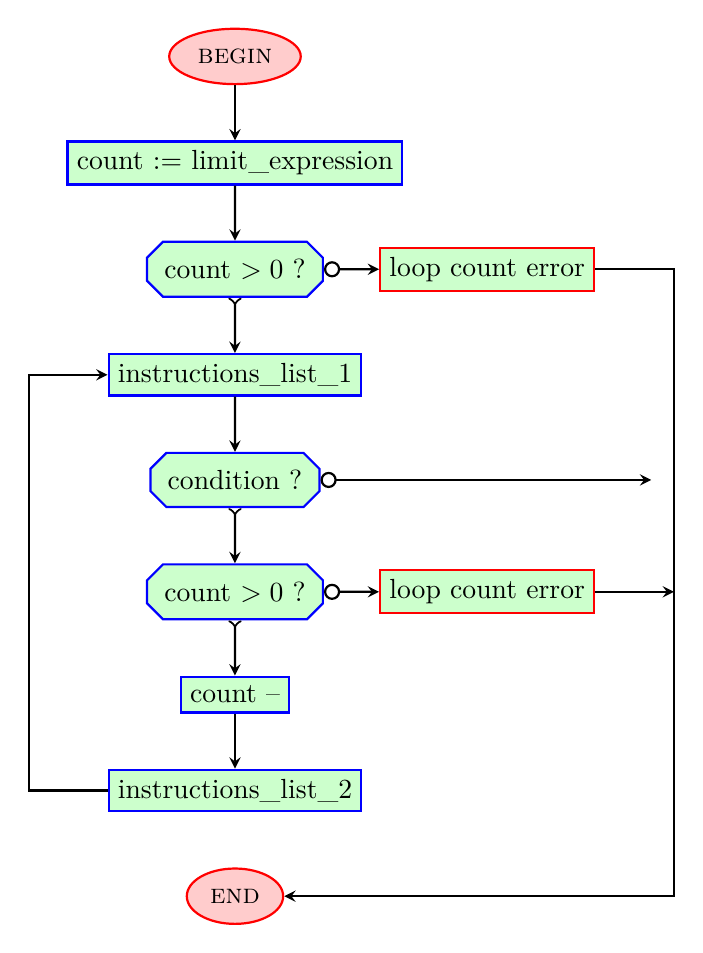
\begin{tikzpicture}[
      cloud/.style ={draw=red, thick, ellipse,fill=red!20, minimum height=2em},
      block/.style ={rectangle, draw=blue, thick, fill=green!20, align=center},
      error/.style ={rectangle, draw=red, thick, fill=green!20, align=center},
      decision/.style={chamfered rectangle, draw=blue, thick, fill=green!20},
      node distance=7mm
    ]
    \node [cloud] (start) {\textsc{begin}} ;
    \node [block] (affectationVariant) [below=of start] {count := {\tt \emph{limit_expression}}} ;
    \node [decision] (premierTest) [below=of affectationVariant]{count $> 0$ ?} ;
    \node [error] (loopVariantError) [right=of premierTest] {loop count error} ;
    \node [block] (instructions1) [below=of premierTest] {\tt \emph{instructions\_list\_1}} ;
    \node [decision] (expression) [below=of instructions1] {\tt \emph{condition} ?} ;
    \node [decision] (secondTest) [below=of expression] {count $> 0$ ?} ;
    \node [error] (loopVariantError2) [right=of secondTest] {loop count error} ;
    \node [block] (decVariant) [below=of secondTest] {count {-}{-}} ;
    \node [block] (instructions2) [below=of decVariant] {\tt \emph{instructions\_list\_2}} ;
    \node [cloud] (end) [below=of instructions2] {\textsc{end}} ;
    
    \draw [-stealth, thick] (start) -- (affectationVariant) ;
    \draw [-stealth, thick] (affectationVariant) -- (premierTest) ;
    \draw [o-stealth, thick] (premierTest) -- (loopVariantError) ;
    \draw [o-stealth, thick] (secondTest) -- (loopVariantError2) ;
    \draw [-stealth, thick] (loopVariantError.east) -- +(1, 0) |- (end.east) ;
    \draw [-stealth, thick] (loopVariantError2.east) -- +(1, 0) ;
    \draw [o-stealth, thick] (expression.east) -- +(4.2, 0) ;
    \draw [-stealth, thick] (instructions1) -- (expression) ;
    \draw [>-stealth, thick] (premierTest) -- (instructions1) ;
    \draw [>-stealth, thick] (expression) -- (secondTest) ;
    \draw [>-stealth, thick] (secondTest) -- (decVariant) ;
    \draw [-stealth, thick] (decVariant) -- (instructions2) ;
    \draw [-stealth, thick] (instructions2.west) -- +(-1, 0) |- (instructions1.west) ;
  \end{tikzpicture}
  }
  \caption{semantics of the \gtlinline{repeat} instruction}
  \label{fig:repeat}
\end{figure}

\example
\begin{gtl}
let aList := @( 1, 2, 3, 4 )
repeat ( [aList length] )
while [aList length] > 0 do
  println [aList first]
  unlet aList[0]
end repeat
\end{gtl}
\begin{console}
1
2
3
4
\end{console}

\section{The \texttt{write} instruction}

The \gtlinline{write} instruction writes the template output string to a file. The general form is:

\begin{gtl}
write to <executable> expression :
  instruction_list
end write
\end{gtl}

Where \gtlinline{expression} is a \gtltype{string} expression. Here the template output string built by instructions in the \gtlinline{instruction_list} are written to the file named after the evaluation of \gtlinline{expression}. 

If the optional keyword \gtlinline{executable} is present, the file has its executable bit set.

\examplen{1}
\begin{gtl}
write to "/tmp/outputOfTemplate" :
%Hello
%
end write
\end{gtl}
\begin{console}
Created '/tmp/outputOfTemplate'.
\end{console}

\noindent The content of file at path \texttt{\small '/tmp/outputOfTemplate'} is:
\begin{templateoutput}
Hello
\end{templateoutput}

\examplen{2}
\begin{gtl}
write to executable "/tmp/listfiles.sh" :
%# /bin/sh
ls -al
%
end write
\end{gtl}
\begin{console}
Created '/tmp/listfiles.sh'.
\end{console}

\noindent The content of file at path \texttt{\small '/tmp/outputOfTemplate'} is:
\begin{templateoutput}
# /bin/sh
ls -al
\end{templateoutput}
And since it is an executable file, one can type \texttt{\small '/tmp/listfiles.sh'} to execute the shell script.

\section{The \texttt{template} instruction}

The \gtlinline{template} instruction invokes another template. The output string built by the invoked template is included in the output string of the caller at the location occupied by the \gtlinline{template} instruction. The general form is:

\begin{gtl}
template <(argument_list)> <if exists> file_reference <in hierarchy>
<or>
  <instruction_list>
<end template> 
\end{gtl}

\subsection{Template invocation with a copy of variables}

The simplest form is:

\begin{gtl}
template file_reference
\end{gtl}

The \gtlinline{file_reference} may be an identifier or \gtlinline{from} followed by an expression that evaluate to a \gtltype{string}.

\begin{gtl}
template aTemplate # identifier file reference
\end{gtl}

\noindent or

\begin{gtl}
template from "aTemplate" # string file reference
\end{gtl}

The second one allow to use any file name. In both cases, the \gtlinline{template} instruction looks for a file named \gtlinline{aTemplate.extension}. \gtlinline{extension} is customizable. For \tool{gtl} it is set to \scst{gtl}. For \tool{goil} it is set to \scst{goilTemplate}.

If the template file is found it get a copy of the variables of the caller and is executed. If it is not found a runtime error occurs.

\example

\noindent Contents of \texttt{\small callerTemplate.gtl}:

\begin{gtl}
loop a from 1 to 4 do
  template helloTemplate 
  % % !a % %
end loop
%
%
\end{gtl}
\noindent Contents of \texttt{\small helloTemplate.gtl}:
\begin{gtl-tmode}
Hello
\end{gtl-tmode}
\begin{templateoutput}
Hello 1 Hello 2 Hello 3 Hello 4 
\end{templateoutput}

\subsection{Template invocation with arguments}
\label{sec:templatesArgs}

Instead of passing a copy of all the variables to the invoked template, it is possible to pass arguments. In this case the invoked template works as a procedure and has no access to the variables of the caller. See \ref{sec:input} too.

\example

\noindent Contents of \texttt{\small caller2Template.gtl}:
\begin{gtl}
loop a from 1 to 4 do
  template (a) hello2Template 
end loop
%
%
\end{gtl}
\noindent Contents of \texttt{\small hello2Template.gtl}:
\begin{gtl}
input(number)
%Hello % !number % %
\end{gtl}

\begin{templateoutput}
Hello 1 Hello 2 Hello 3 Hello 4 
\end{templateoutput}

\subsection{Conditional invocation of templates}

In some cases, the invocation of a template may be optional and if the template is not found, no error should occurs. The following form goes this:

\begin{gtl}
template if exists file_reference
\end{gtl}

If the template file is found it get a copy of the variables of the caller and is executed. If it is not found the template invocation fails silently.

When the template file is not found it is possible to execute a list of instructions. This is done by adding a \gtlinline{or}, the instruction list and \gtlinline{end template}.

\begin{gtl}
template if exists file_reference or
  instruction_list
end template
\end{gtl}

\section{The \texttt{input} instruction}
\label{sec:input}

The \gtlinline{input} instruction is used in a template to retrieve the arguments passed to the template by the caller. See section \ref{sec:templatesArgs}

\begin{gtl}
input(formal_argument_list)
\end{gtl}

\gtlinline{input} may be used at any time in the template. For each variable appearing in the \gtlinline{formal_argument_list} input pops the first value from the argument list passed by the caller. This can be done by one or more \gtlinline{input} instructions.

\example
\begin{gtl}
# The caller invoke a template with argument 1, 2, 3 and 4
template (1, 2, 3, 4) aTemplate
\end{gtl}
\noindent Contents of file \texttt{\small aTemplate.gtl}:
\begin{gtl}
input(a)    # retrieve 1
input(b, c) # retrieve 2 in b and 3 in c
input(d)    # retrieve 4
input(e)    # trigger a runtime error, the argument list is empty
\end{gtl}

Arguments in the \gtlinline{formal_argument_list} may be typed. In the following example any data type may be passed for \gtlinline{d} but \gtlinline{c} requires an \gtltype{int} and \gtlinline{a} requires a \gtltype{string}.

\example
\begin{gtl}
template (3, 2, 1) aTemplate
\end{gtl}
\noindent Contents of file \texttt{\small aTemplate.gtl}:
\begin{gtl}
input(c : @int, d) # retrieve 3 in c and 2 in d
input(a : @string) # trigger an error int 1 is not a string
\end{gtl}

\section{The \texttt{error} and \texttt{warning} instructions}
\label{sec:errorInstruction}
\label{sec:warningInstruction}

It can be useful to generate an error or a warning if a data is not defined or if its value is unappropriate.  \gtlinline{error} and \gtlinline{warning} have 2 forms:

\begin{gtl}
error var : expression
warning var : expression
\end{gtl}

\noindent or

\begin{gtl}
error here : expression
warning here : expression
\end{gtl}

\gtlinline{expression} must be of type \gtltype{string}. In the first form, \gtlinline{var} is a  variable. The file location of this variable may be a location in any input file of the compiler which embeds the GTL interpreter or in the template file if the variable was assigned in the template. This location is used to signal the location of the error or warning. In the second form, \gtlinline{here} means the current location in the template file.

In the following example taken from the Goil templates, an error is generated if the \texttt{\footnotesize ACTIVATION} attribute of an extended task is greater than \icst{1}:

\examplen{1}
\begin{gtl}
# Check no extended task as an ACTIVATION attribute greater than 1
foreach task in EXTENDEDTASKS do
  if task::ACTIVATION > 1 then
    error task::ACTIVATION : "An extended task cannot have ACTIVATION greater than 1"
  end if
end foreach
\end{gtl}

In this second example, a warning is generated if a template is not found:

\examplen{2}
\begin{gtl}
template if exists interrupt_wrapping or
  warning here : "interrupt_wrapping.goilTemplate not found"
end template
\end{gtl}

\section{The \texttt{print} and \texttt{println} instructions}

\gtlinline{print} an \gtlinline{println} print an \gtlinline{expression} to the standard output. \gtlinline{println} prints a \ccst{\textbackslash n} after the expression. \gtlinline{println} may be used alone to print a \ccst{\textbackslash n}.

\begin{gtl}
print expression
println <expression>
\end{gtl}

Any \gtltype{string}, \gtltype{int}, \gtltype{bool}, \gtltype{float}, \gtltype{enum}, \gtltype{type} and \gtltype{char} may be printed. \gtltype{struct}, \gtltype{list}, \gtltype{map} and \gtltype{unconstructed} may not.

\example
\begin{gtl}
foreach a in @( "Does", "anybody", "remember", "Vera", "Lynn", '?' ) do
  print a 
  print " "
end foreach
println
\end{gtl}
\begin{console}
Does anybody remember Vera Lynn ? 
\end{console}

\section{The \texttt{display} instruction}

\gtlinline{display} prints the name of any variable, the location of the \gtlinline{display} instruction and the content of any variable. It is designed to be use for debug purpose. To get the following output, a \gtlinline{display TASKS} has been added to \texttt{\footnotesize root.goilTemplate} and the example in \texttt{\footnotesize examples/cortex/\-armv7em/stm32f407/stm32f4discovery/alarms} has been compiled by Goil.

\example
\begin{console}
TASKS from file '/Users/jlb/Develop/trampoline-git-maintain/goil/templates/root.goilTemplate', line 1467:7
  - list: @(
    0 :>
        struct: @{
            ACTIVATION :>
                integer: 1
            AUTOSTART :>
                boolean: false
            KIND :>
                string: "Task"
            NAME :>
                string: "blink"
            NONPREEMPTABLE :>
                boolean: false
            PRIORITY :>
                integer: 1
            SCHEDULE :>
                string: "FULL"
            STACKSIZE :>
                integer: 300
            USEFLOAT :>
                boolean: false
            USEINTERNALRESOURCE :>
                boolean: false
        }
    1 :>
        struct: @{
            ACTIVATION :>
                integer: 1
            AUTOSTART :>
                boolean: false
            KIND :>
                string: "Task"
            NAME :>
                string: "read_button"
            NONPREEMPTABLE :>
                boolean: false
            PRIORITY :>
                integer: 2
            SCHEDULE :>
                string: "FULL"
            STACKSIZE :>
                integer: 300
            USEFLOAT :>
                boolean: false
            USEINTERNALRESOURCE :>
                boolean: false
        }
)
\end{console}

\section{The \texttt{variables} instruction}

\gtlinline{variables} displays all the variables. It is designed to be use for debug purpose.

\begin{gtl}
variables
\end{gtl}

\example
\begin{gtl}
let a := @( 1, 2, 3 )
let b := @{ x:1, y:2, z:3 }
let c := @[ "age": 10, "name": "Vera" ]
let d := "Hello"
let e := 3
variables
\end{gtl}
\begin{console}
================= Variables ================== Displayed from =================
file '/Users/jlb/Develop/GTL/examples/variables.gtl', line 7:9
===============================================================================
-------------------------------------------------------------------------------
a
-------------------------------------------------------------------------------
list: @(
    0 :>
        integer: 1
    1 :>
        integer: 2
    2 :>
        integer: 3
)
-------------------------------------------------------------------------------
b
-------------------------------------------------------------------------------
struct: @{
    x :>
        integer: 1
    y :>
        integer: 2
    z :>
        integer: 3
}
-------------------------------------------------------------------------------
c
-------------------------------------------------------------------------------
map: @[
    "age" :>
        integer: 10
    "name" :>
        string: "Vera"
]
-------------------------------------------------------------------------------
d
-------------------------------------------------------------------------------
string: "Hello"
-------------------------------------------------------------------------------
e
-------------------------------------------------------------------------------
integer: 3
===============================================================================
\end{console}

\chapter{GTL modules}

GTL may be extended with functions, setters and getters. Definitions of these objects are done in  separates \texttt{\footnotesize .gtm} files called modules.

\section{Importing a module}

Modules are imported by using the \gtlinline{import} statement. GTL prevents multiple import of the same module.

\begin{gtl}
import expression
\end{gtl}

\gtlinline{expression} must evaluate to a \gtltype{string}. \gtlinline{import} is not an instruction and must appear at the beginning of the template file before any instruction except the \gtlinline{\%...\%} instruction.

\section{Writing a module}

A module includes zero or more functions definitions, zero or more getter definitions and zero or more setter definitions. It may include \gtlinline{import} statements too but they must appear before any function~/ getter~/ setter definition. If  \gtlinline{\%...\%} instructions are used they are ignored. Other instructions which output data in the output template string are forbidden.

\subsection{The arguments}

Arguments are passed by copy. Each formal argument of the list may be typed or not. If a formal argument is typed, GTL emit a runtime error if the passed argument does not have the same type. Here is a formal argument list with the second argument typed.

\begin{gtl}
a, b : @int, c
\end{gtl}

Any data type may be passed for arguments \gtlinline{a} and \gtlinline{c} but an \gtltype{int} is required for argument \gtlinline{c}.

The type of an argument may be tested, check \ref{sec:type}, \ref{sec:isANumber} and \ref{sec:function}.

\subsection{Function definition}
\label{sec:function}

A function definition has the following form:

\begin{gtl}
func func_name(formal_argument_list) result_var
  instruction_list
end func
\end{gtl}

The \gtlinline{formal_argument_list} may be empty. \gtlinline{result_var} is a local variable of the function which is used to return the result.

\examplen{1}

\noindent Content of \texttt{\footnotesize function.gtm}:
\begin{gtl}
func square(x) result
  let result := x * x
end func
\end{gtl}
\noindent Content of \texttt{\footnotesize template.gtl}:
\begin{gtl}
import "function"

let b := square(6)
display b
let b := square(2.6)
display b
\end{gtl}
\begin{console}
b from file '/Users/jlb/Develop/GTL/examples/template.gtl', line 5:7
  - integer: 36
b from file '/Users/jlb/Develop/GTL/examples/template.gtl', line 7:7
  - float: 6.76
\end{console}

\examplen{2}

\noindent Content of \texttt{\footnotesize function.gtm}:
\begin{gtl}
func square(x : @int) result
  let result := x * x
end func
\end{gtl}
\noindent Content of \texttt{\footnotesize template.gtl}:
\begin{gtl}
import "function"

let b := square(6)
display b
let b := square(2.6)
display b
\end{gtl}
\begin{console}
b from file '/Users/jlb/Develop/GTL/examples/template.gtl', line 5:7
  - integer: 36
/Users/jlb/Develop/GTL/examples/template.gtl:6:17:19:
semantic error #1: int expected for x
let b := square(2.6)
----------------^^^
\end{console}

\examplen{3}

\noindent Content of \texttt{\footnotesize function.gtm}:
\begin{gtl}
func square(x) result
  if [x isANumber] then
    let result := x * x
  else
    error here : "int or float expected"
  end if
end func
\end{gtl}
\noindent Content of \texttt{\footnotesize template.gtl}:
\begin{gtl}
import "function"

let b := square(6)
display b
let b := square(2.6)
display b
let b := square("Hello")
display b
\end{gtl}
\begin{console}
b from file '/Users/jlb/Develop/GTL/examples/template.gtl', line 5:7
  - integer: 36
b from file '/Users/jlb/Develop/GTL/examples/template.gtl', line 7:7
  - float: 6.76
/Users/jlb/Develop/GTL/examples/template.gtl:6:18:24:
semantic error #1: int or float expected
let b := psquare("Hello")
-----------------^^^^^^^
\end{console}

\section{Getter definition}
\label{sec:getter}

A getter is defined as follow:

\begin{gtl}
getter a_type getter_name(formal_argument_list) result_var
  instruction_list
end getter
\end{gtl}

\gtlinline{a_type} designates the data type on which the getter apply. It can be \gtlinline{@int},  \gtlinline{@char}, \gtlinline{@float}, \gtlinline{@bool}, \gtlinline{	@enum}, \gtlinline{@string}, \gtlinline{@struct}, \gtlinline{@list}, \gtlinline{@map}, \gtlinline{@type} or \gtlinline{@unconstructed}. \gtlinline{getter_name} is the name of the getter. The same name may be used for several types. The \gtlinline{formal_argument_list} follows the same rules as those exposed in \ref{sec:function}. \gtlinline{result_var} is the name of the variable used to store the result of the getter.

Within the getter, variable \gtlinline{self} is a copy of the variable targeted by the getter. It can me modified but the target will not be touched.

\examplen{1}

In this example a getter to get the square of an \gtltype{int} is defined

\noindent Content of \texttt{\footnotesize getter.gtm}:
\begin{gtl}
#----------------------------------------------------------------
# getter : square of a int
#----------------------------------------------------------------
getter @int square() result
  let result := self * self
end getter
\end{gtl}
\noindent Content of \texttt{\footnotesize template.gtl}:
\begin{gtl}
import "getter"

let b := [6 square]
display b
let b := [b square]
display b
\end{gtl}
\begin{console}
b from file '/Users/jlb/Develop/GTL/examples/testGetter.gtl', line 5:7
  - integer: 36
b from file '/Users/jlb/Develop/GTL/examples/testGetter.gtl', line 7:7
  - integer: 1296
\end{console}

\examplen{2}

In this example two getters, one to check a \gtltype{struct} and the other to check a \gtltype{list} are defined

\noindent Content of \texttt{\footnotesize getter.gtm}:
\begin{gtl}
#----------------------------------------------------------------
# getter : returns true if the target has a field
#----------------------------------------------------------------
getter @struct hasField(field : @string) result
  let selfAsMap := [self map]
  let result := exists selfAsMap[field]
end getter


#----------------------------------------------------------------
# getter : returns true if all the elements of the list are
# structs and if all the elements of the list have a field
#----------------------------------------------------------------
getter @list alwaysHasField(field : @string) result
  let result := true
  foreach element in self do
    let result &= [element hasField : field]
  end foreach
end getter
\end{gtl}
\noindent Content of \texttt{\footnotesize template.gtl}:
\begin{gtl}
let c := @(
  @{ age : 18, height : 180, name : "Arnold" },
  @{ age : 22, height : 170, name : "Bob"    },
  @{ age : 29, height : 175, name : "John"   }
)

if [c alwaysHasField : "age"] then
  println "List 1 ok"
else
  println "List 1 ko"
end if

let c += @{ height : 150, name : "Sally" }

if [c alwaysHasField : "age"] then
  println "List 2 ok"
else
  println "List 2 ko"
end if
\end{gtl}
\begin{console}
List 1 ok
List 2 ko
\end{console}

\section{Setter definition}

A setter is defined as follow:

\begin{gtl}
setter a_type setter_name(formal_argument_list)
  instruction_list
end getter
\end{gtl}

\gtlinline{a_type} designates the data type on which the setter apply. It can be \gtlinline{@int},  \gtlinline{@char}, \gtlinline{@float}, \gtlinline{@bool}, \gtlinline{	@enum}, \gtlinline{@string}, \gtlinline{@struct}, \gtlinline{@list}, \gtlinline{@map}, \gtlinline{@type} or \gtlinline{@unconstructed}. \gtlinline{setter_name} is the name of the setter. The same name may be used for several types. The \gtlinline{formal_argument_list} follows the same rules as those exposed in \ref{sec:function}.

Within the setter, variable \gtlinline{self} is the variable targeted by the setter.

\example

\noindent Content of \texttt{\footnotesize setter.gtm}:
\begin{gtl}
#----------------------------------------------------------------
# setter : delete all list items which are struct and with a
# field named age
#----------------------------------------------------------------
setter @list deleteAge()
  let theList := self
  let offset := 0
  foreach element (index) in theList do
    if exists element::age then
      unlet self[index + offset]
      let offset -= 1
    end if
  end foreach
end setter
\end{gtl}

\noindent Content of \texttt{\footnotesize template.gtl}:
\begin{gtl}
let c := @(
  @{ age : 18, height : 180, name : "Arnold" },
  @{ age : 22, height : 170, name : "Bob"    },
  @{ age : 29, height : 175, name : "John"   },
  @{           height : 150, name : "Sally"  }
)

[!c deleteAge]
display c
\end{gtl}
\begin{console}
c from file '/Users/jlb/Develop/GTL/examples/template.gtl', line 36:7
  - list: @(
    0 :>
        struct: @{
            height :>
                integer: 150
            name :>
                string: "Sally"
        }
)
\end{console}

\end{document}  